

\chapter{Construcción de un modelo general de predicción de la gravedad de un accidente de tráfico}

En este capítulo se describe el proceso para el desarrollo de un modelo general de predicción de gravedad de accidentes de tráfico aplicable a cualquier región e independiente a los datos que puedan estar disponibles en cada una de ellas. Para llegar a este fin, inicialmente se realizó una investigación y se implementó un primer modelo a modo de prototipo sobre el que aplicar modificaciones e hipótesis hasta llegar al objetivo final, un procedimiento que no fuese sensible a la disponibilidad de datos y fuera independiente de la región sobre la que se aplicase, es decir, un modelo general de predicción de la necesidad de asistencia en los accidentes de tráfico general. Por este motivo, este apartado se divide en dos subsecciones. La primera de ella describe la intuición sobre el primer prototipo, describiendo brevemente las fases que lo componen, los objetivos finales de este, incidiendo en las partes que han evolucionado respecto al modelo final. La siguiente sección de este apartado expone el modelo final tras la evolución del prototipo como referencia, justificando las decisiones tomadas en cada caso.

% \textcolor{blue}{\textbf{Luis: esta intro y todo el punto del modelo preeliminar no me termina de convencer, lo hablamos cuando podais.}}\\

\section{Modelo preliminar}
\label{METODOLOGIA_MODELO_PRELIMINAR}

%\sout{\textcolor{red}{MANU: En una primera fase de la tesis doctoral, se propuso un modelo preliminar aplicado a un dataset concreto, orientado a la gravedad del accidente, estableciendo una clasificación de 3 niveles (leve, severo y fatal). Con el objetivo principal de la tesis de realizar un modelo general y la reclasificación del problema a la necesidad de asistencia en un accidente de tráfico, se explica en este apartado brevemente el modelo preliminar, y explicado con total detalle en la siguiente sección 4.3 el modelo general que se propone.}}


En una primera fase de la investigación, se propuso un modelo preliminar de predicción de la gravedad de accidentes de tráfico aplicado a una ciudad \cite{PEREZSALA2023113245}, teniendo como meta la predicción de la gravedad de los accidentes en base a 3 niveles (leve, severo y fatal). Como el objetivo de este trabajo es diseñar un modelo predictivo general a cualquier ciudad, en este apartado se expondrá brevemente el enfoque del modelo preliminar,a modo de introducción y acentuando los matices que condujeron a la reclasificación posterior de las clases que describían la necesidad de asistencia. El modelo general que se propone se explicará con total detalle en la siguiente sección \ref{METODOLOGIA_GTAAF}.

Este primer prototipo se presentó en \cite{PEREZSALA2023113245} y se implementó con el objetivo de predecir la gravedad de los accidentes de tráfico utilizando un dataset de la ciudad de Madrid. Concretamente, se dividió la gravedad de los accidentes entres categorías distintas que estaban en ese conjunto de datos: (1) Leves, (2) Severos y (3) Fatales.

Para llegar al entrenamiento de un clasificador predictivo, se diseñó un modelo compuesto por cinco fases secuenciales, mostradas en la Figura \ref{figDegree}, teniendo como objetivo realizar transformaciones y operaciones sobre datos, inicialmente tabulares, para transformarlos en datos matriciales sobre los que pudieran operar modelos diseñados para tratar imágenes. De esta forma era posible experimentar con dos modelos convolucionales, el primero de ellos unidimensional y el segundo bidimensional, CNN-1D y CNN-2D respectivamente.

Primeramente fue necesario definir una categorización de características, las cuales fueron utilizadas como apoyo para la construcción de estas matrices. Para la construcción de las matrices que alimentan las redes convolucionales se le asignó una importancia a cada variable dentro del conjunto de datos con la finalidad de situarlas en determinados lugares de estas matrices. Es decir, dependiendo de la importancia asignada a cada variable, se le asignaba una posición en la matriz. 

Finalmente los modelos convolucionales propuestos se compararon con otros tres modelos del estado del arte \textit{(Naive Bayes, Support Vector Classifier y k-Nearest Neighbor)} para evaluar sus rendimientos respectivos en el dataset de la ciudad de Madrid.

En la figura \ref{figDegree} se enumeran las etapas que definen el flujo del modelo preliminar prototipo.

\begin{figure}[h]
	\centering
	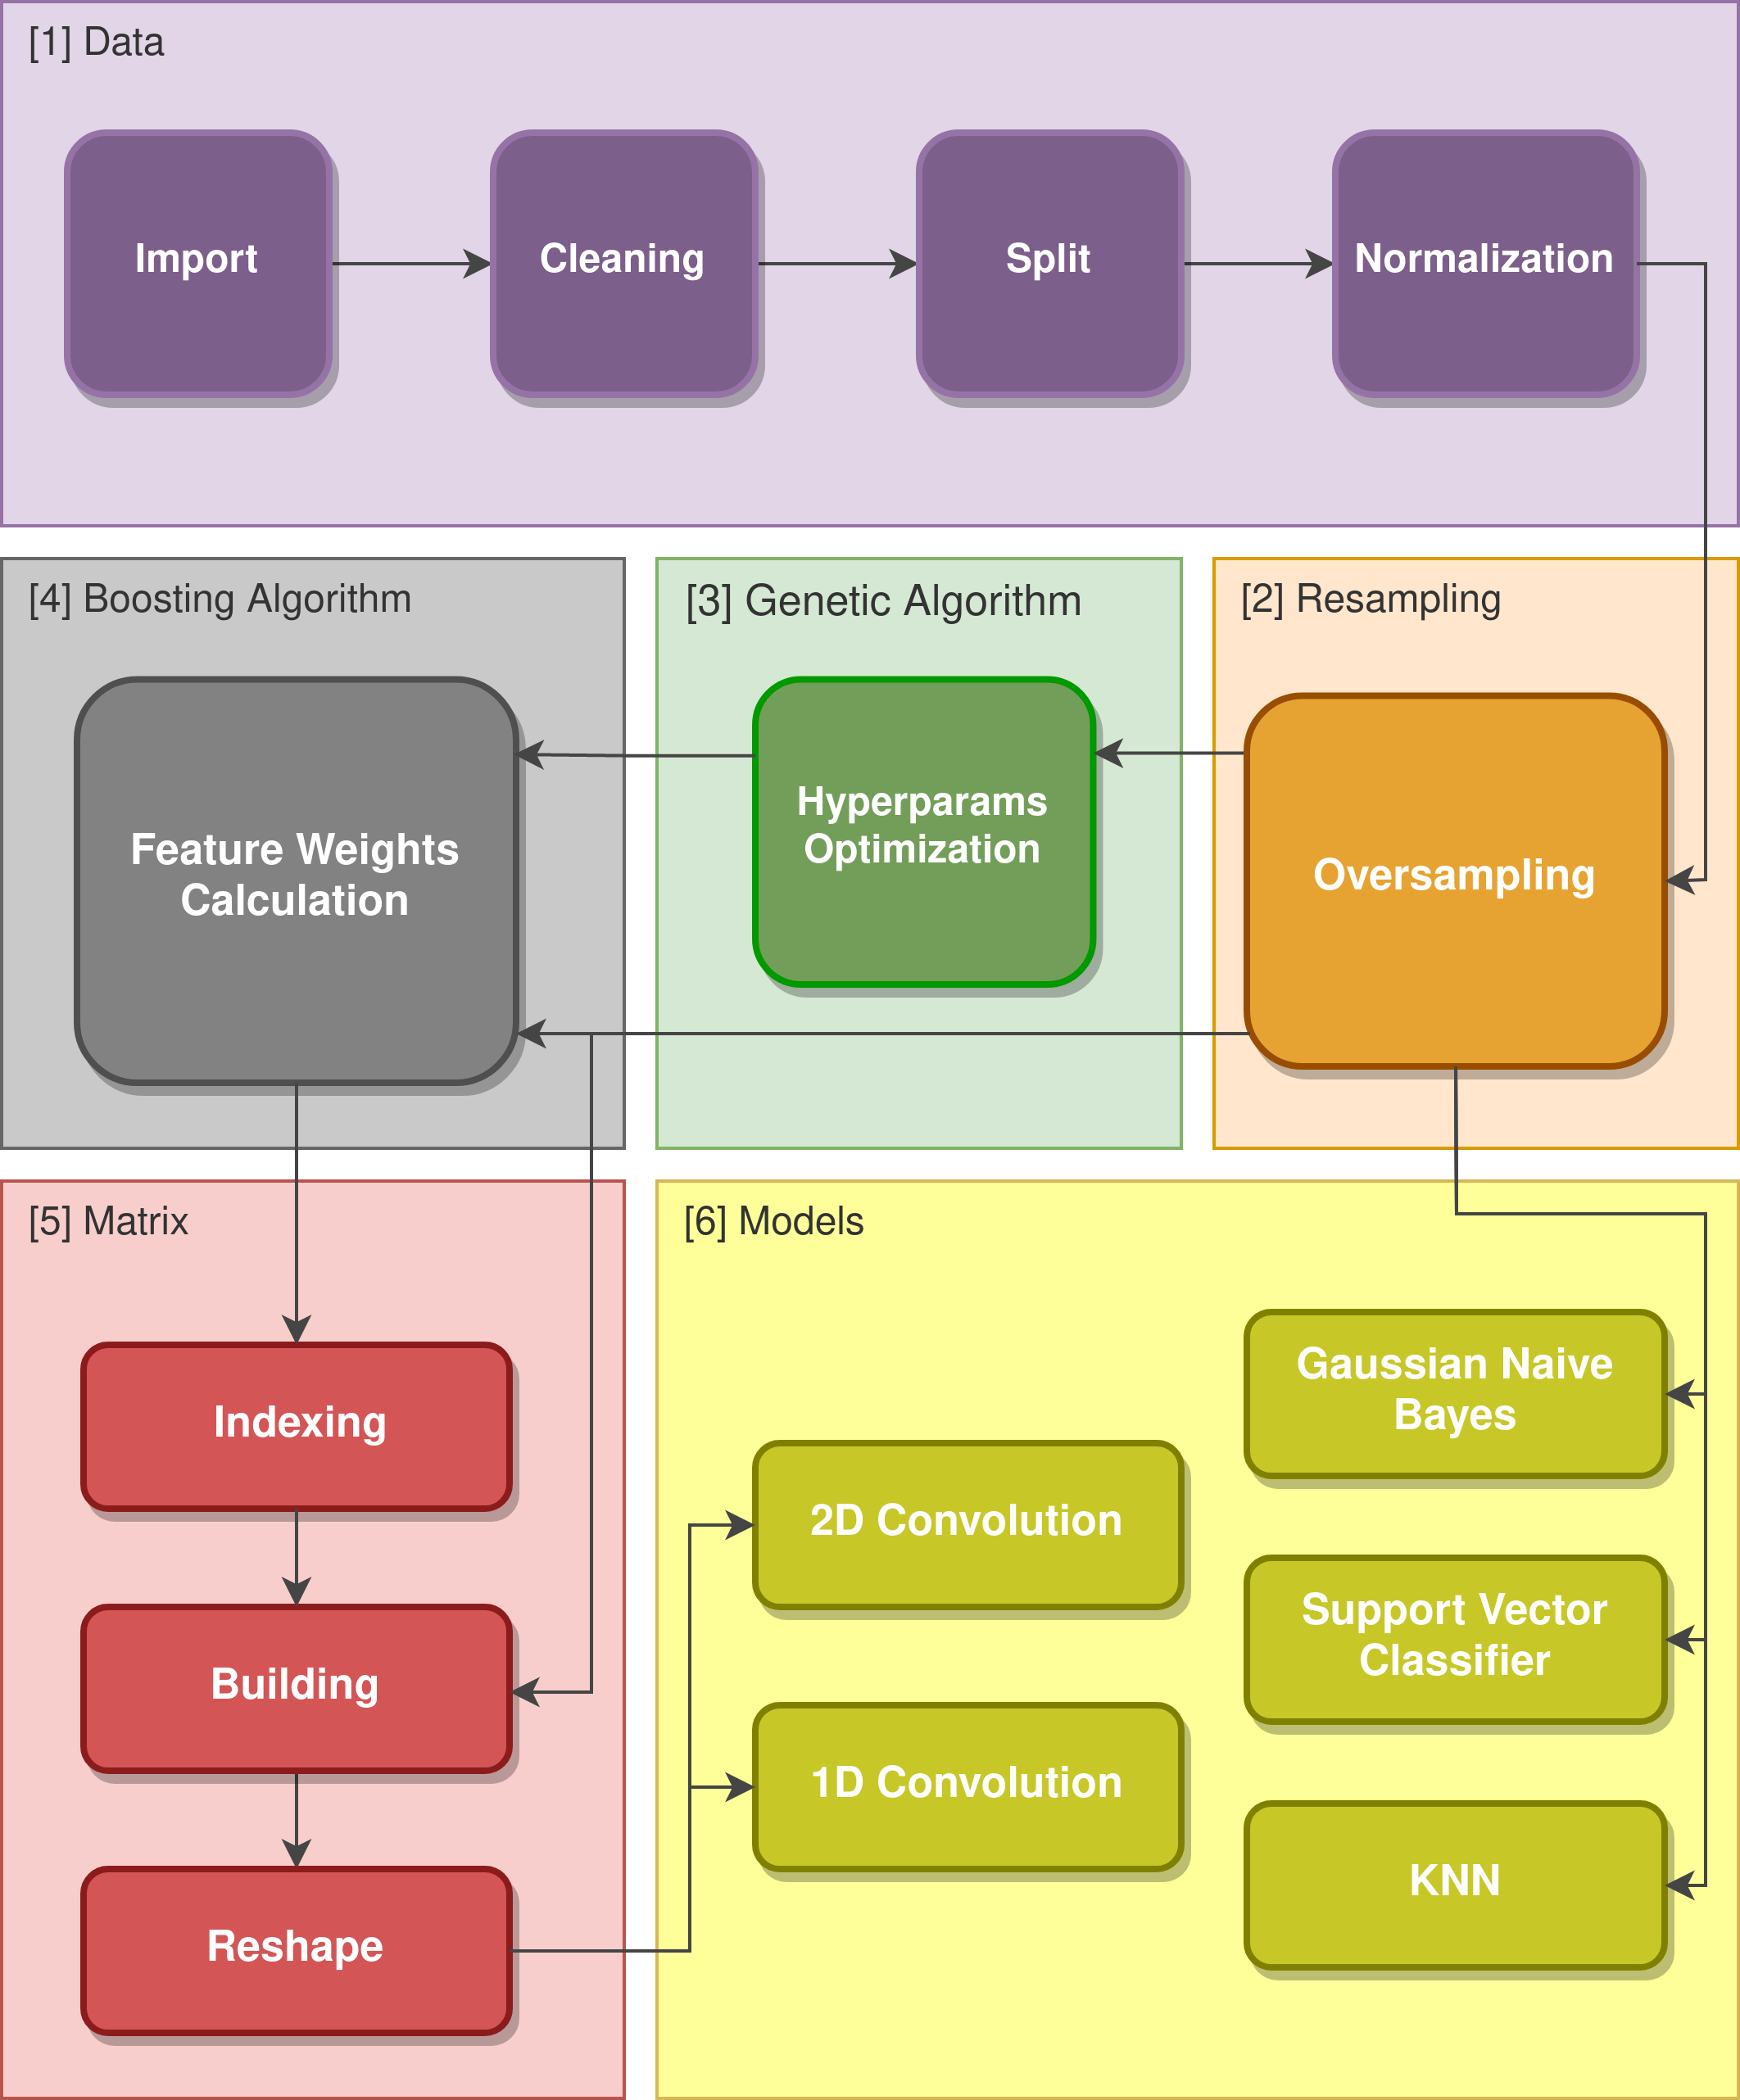
\includegraphics[width=3.5in]{Figures/1stPaper/Data_flow.png}
	\caption{Diagrama de flujo del modelo preliminar propuesto}
	\label{figDegree}
\end{figure}

La primera fase (1) en la Figura \ref{figDegree}, está orientada al tratamiento de los datos. Los datos originales del dataset eran datos en bruto, donde se podían encontrar errores en los valores, valores atípicos y variables con valores cualitativos que había que discretizar. Es por esto que en esta etapa se diseñaron métodos para tratar estos datos, concretamente aplicándoles un proceso de limpieza, una discretización para que fuesen interpretables por los modelos, un tratamiento para su normalización y otro para evitar que estuviesen sobredimensionados.

En una segunda fase (2), se aplicó un proceso para trabajar sobre el desbalanceo de los datos presente el dataset ya que, debido a la naturaleza de los accidentes de tráfico, gran parte de ellos eran de tipo leve, mientras que el resto de accidentes (severos y fatales), presentaban una proporción mucho menor. Para evitar un sesgo en los modelos, es decir, una tendencia a predecir cualquier nueva muestra como accidente tipo leve (la de clase mayoritaria), se estudiaron distintas técnicas de balanceo de datos. Finalmente, se utilizó la técnica \textit{Borderline SMOTE-II} para balancear las clases minoritarias, aplicando generación de datos sintéticos para igualar el número de muestras de las otras dos clases hasta llegar a la mayoritaria.

Una tercera fase (3) buscaba transformar los datos tabulares resultantes a datos matriciales interpretables por los modelos convolucionales. Para esto se requería de algún tipo de estrategia para la asignación de cada una de las variables del dataset a coordenadas dentro de una matriz bidimensional con el objetivo de aplicar los modelos convolucionales propuestos en este prototipo. Para llevar a cabo esto, se tomó una estrategia que requería de conocer la importancia de cada variable dentro del conjunto de datos. Como método para hallar el peso de cada característica dentro del dataset se utilizó un algoritmo tipo \textit{Boosting}. Los algoritmos tipo \textit{Boosting} son clasificadores que ofrecen la importancia numérica de cada variable en función del peso que han tenido durante su entrenamiento. Estos algoritmos necesitan una configuración de hiperparámetros que se optimizaron mediante la evolución de las posibles configuraciones a través de un algoritmo genético (4).

Una vez se disponían de los pesos de las características gracias al cálculo del algoritmo tipo \textit{Boosting} (5), se categorizaron las variables en distintas categorías (6) para tener una referencia bidimensional sobre la que comenzar a asignar las variables. En primer lugar se calculó el peso total de las categorías, que era la suma de los pesos de cada una de las variables que contenía. Como resultado de esto, cada categoría se indexaba a una fila de la matriz, donde aquella que más peso presentaba era asignada a la fila central, la segunda en la posición inmediatamente superior, la siguiente en la inferior y así sucesivamente. Por otro lado, las características que las componían se asociaban a las columnas dentro de su categoría de forma similar, la de mayor peso en la posición central, la siguiente en su posición inmediatamente a la izquierda, la siguiente a la derecha, etc. Como resultado de este proceso, cada registro perteneciente al dataset original era transformado en una matriz de tamaño $5\times5$.

Las arquitecturas que se propusieron en la fase prototipo eran dos redes convolucionales, de una y dos dimensiones. Estas constaban de cuatro capas convolucionales con tamaños de \textit{kernels}, de $(1 \times 3)$ para la CNN-1D, y $(3 \times 3)$ para la CNN-2D respectivamente. Estos \textit{kernels} se proyectaban en $256$ y $512$ canales para formar el filtro convolucional asociado con cada capa. Posteriormente se aplicaba un proceso de normalización de batch a la salida de cada uno de los mapas de características. El \textit{padding} de los \textit{kernels} estableció en $1$ para ambos tipos de redes, de modo que las convoluciones se aplicaban agregando ceros a los límites de las matrices, de $1$ para la CNN-1D y ${1, 1}$ para la CNN-2D. Por lo tanto, el desplazamiento de los núcleos se realizaba elemento a elemento en ambas redes. En la salida de cada capa convolucional, se aplicaba la función de activación \textit{Rectified Linear Unit (ReLU)}. La salida de la última capa de convolución transformaba los mapas de características generados de tamaño $5 \times 5$ a un vector unidimensional de $1 \times 25$. A continuación, se aplicaba una capa densa que conectaba cada uno de los $25$ nodos de la capa aplanada con los $128$ nodos de la capa densa, que generaba los \textit{logits} antes de aplicar la última función de activación \textit{Softmax} que devolvía la clase predicha. En la figura \ref{TASPCNNIMAGE} se observa el diseño de la arquitectura de la red propuesta CNN-2D.

\begin{figure}[H]
	\centering
	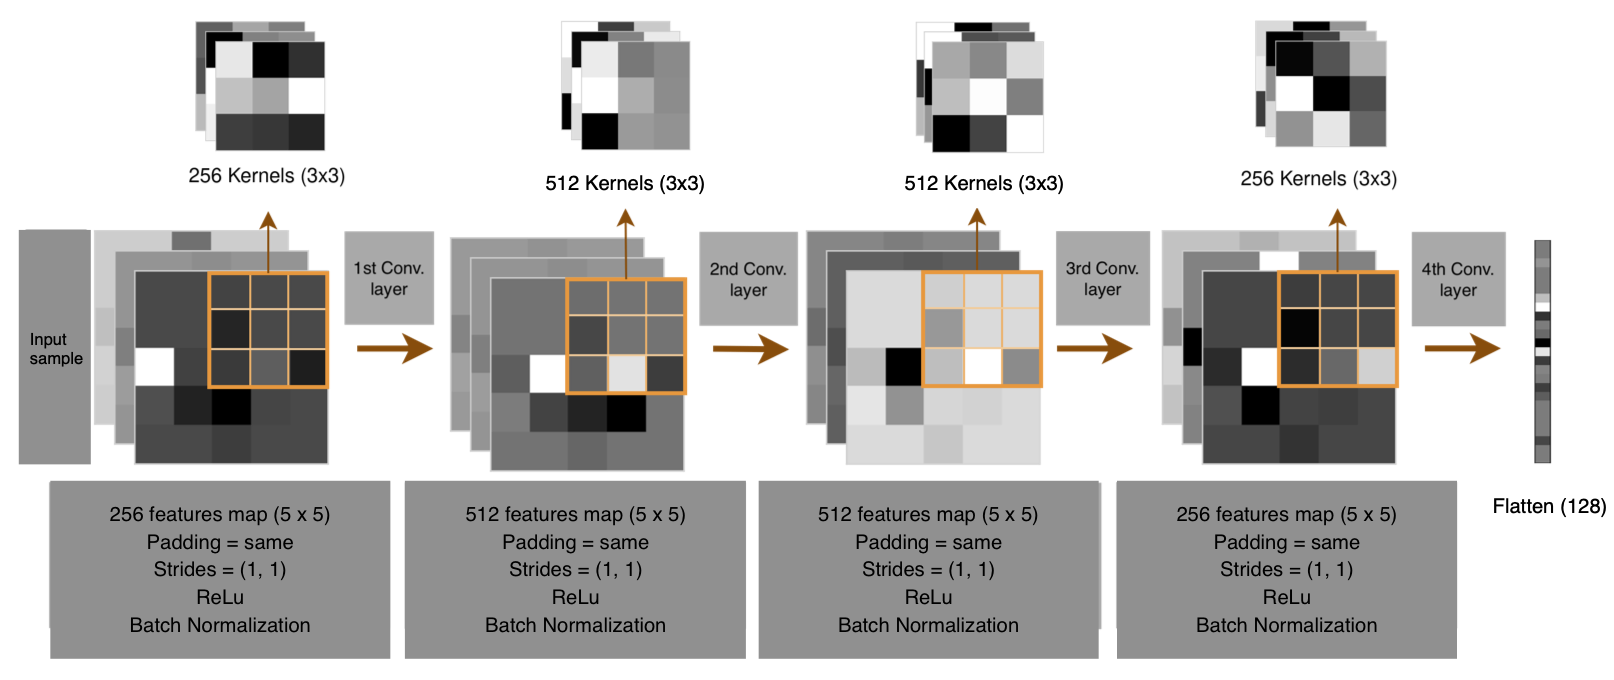
\includegraphics[width=12cm]{Figures/1stPaper/TASPCNN.png}
	\caption{Arquitectura de la red neuronal convolucional 2D}
	\label{TASPCNNIMAGE}
\end{figure}

En última instancia (6), los dos modelos propuestos, CNN-1D y CNN-2D se compararon contra tres modelos del estado del arte, utilizando como referencia de generalización el indicador \textit{F1-Score} sobre conjuntos de datos de test.


\subsubsection*{Aprendizaje resultante del prototipo}

% \underline{Aquí voy a poner las intuiciones de mejora, luego en GTAAF pongo las soluciones a estos problemas?}

Una vez aplicado el modelo sobre el conjunto de datos de Madrid, se analizaron los resultados que este ofrecía sobre el conjunto de datos de test. Esto sirvió para observar ciertas debilidades y localizar puntos de mejora que podrían aumentar el rendimiento de cara a implementar un modelo generalizable a cualquier región.

En primer lugar, se observó que la decisión de dividir los accidentes de tráfico en tres clases (leves, severos y fatales) era un condicionante que perjudicaba considerablemente el rendimiento del modelo. Al tener dos clases notablemente desproporcionadas respecto a la mayoritaria, la generación de datos sintéticos podría carecer de sentido a nivel práctico. Esto hizo que se pensara en agrupar los accidentes en dos categorías (1: leves y 2: graves y fatales) con la finalidad de mejorar el rendimiento del modelo a nivel funcional al no disponer de clases intermedias además de capturar más información al sumar dos tipos de clases.

% El siguiente paso para resolver esto fue la categorización de estos accidentes en dos clases, además de implementar un proceso de filtrado de áreas que uscaba rebajar el número de accidentes tipo leve de forma natural en el conjunto de datos.

Al observarse incongruencias en la interpretación sobre los valores numéricos asignados a determinadas variables, se plantearon cuestiones sobre la discretización de los datos y su inclusión en áreas geolocalizadas. Además, observando las curvas de aprendizaje en las gráficas de entrenamiento de los modelos, se propuso la de mejora de añadir más características a la matriz de entrada a las redes convolucionales, planteándose la inclusión de más variables que pudiesen ser obtenidas en base a transformaciones sobre los datos existentes para aportar más información al modelo.

\section{Modelo GTAAF}
\label{METODOLOGIA_GTAAF}

% \textbf{Luis: aquí de alguna forma te tienes que traer la categorización de la sección de resultados, para decir que la metodología generalizable se usa en base a esto.}\\
%\textcolor{red}{Luis: este párrafo inical entra en colapso con la sección de Resultados 1.1.1 Descripción de datos, se dicen cosas muy parecidas. Hay que analizar cuál nos gusta más y reestructurarlo}
%\textcolor{purple}{\textbf{Jose:} No estra en colapso con nada, si se repite dos veces no pasa nada...}
%\textcolor{orange}{\textbf{Luis: } vale, gracias Jose.}

% \textcolor{orange}{\textbf{Luis: Me parece muy circular todo esto, todo el rato diciendo lo mismo. Opiniones?}}

Después de analizar los resultados ofrecidos del primer prototipo, se propusieron una serie de modificaciones en el modelo enfocadas a mejorar las debilidades observadas. Estos cambios se estructuraron en un nuevo modelo denominado GTAAF (General Model for Traffic Accident Assistance Forecasting) que busca incrementar el rendimiento del prototipo y cuyo principal objetivo es diseñar e implementar un procedimiento de predicción de asistencia de accidentes de tráfico generalizable a cualquier conjunto de datos y región. 

El principal problema observado en los conjuntos de datos de accidentes de tráfico es que, dependiendo de la región y/o gobierno que los ofrezca, estos disponen de información diferente, debido principalmente al coste que supone obtener ciertos datos y a la naturaleza social de la población. Es por esto que, la implementación de un modelo de predicción de necesidad de asistencia en accidentes de tráfico general, requiere un trabajo de análisis de la categorización de las variables disponibles y cuáles pueden ser influyentes en la necesidad de asistencia.

Con la finalidad de solventar estos problemas y presentar una generalización del modelo que sea independiente de los datos disponibles, el modelo GTAAF propuesto se basa en categorización de las características disponibles individuales dependientes de cada conjunto de datos. Así, en función de la naturaleza a la que pertenezca cada dato disponible estos puedan ser asignados a una de las categorías propuestas en este modelo, cuyas propiedades son de fácil adquisición. Esto sortea las peculiaridades individuales de la disponibilidad de datos de cualquier región. 

Para evaluar la eficacia del modelo GTAAF, se compara con otros seis modelos del estado del arte a lo largo de ocho regiones distintas en las mismas condiciones.

En esta sección se explicará con detalle, cada una de las etapas por las que pasan los datos, la justificación de las decisiones tomadas para la construcción de este modelo y las principales diferencias entre la versión preliminar y la versión final.

En primera instancia, las fases del nuevo modelo son asignadas a tres etapas claramente diferenciadas: (en naranja en la Figura \ref{DataFlow}) la fase de Pre-procesamiento, donde se contemplan procesos de limpieza de datos, transformación y balanceo de datos, (en gris) la fase de Postprocesado donde se aplican técnicas de transformación para representar los datos de accidentes en formato tabular a formato matricial, y (en azul) la fase de entrenamiento, donde se entrenará un modelo neuronal convolucional en base a esta representación para predecir la necesidad de asistencia en los accidentes. En la figura \ref{DataFlow} se muestran, en modo de diagrama, cada una de las fases que componen el modelo GTAAF.

\begin{figure}[H]
	\centering
	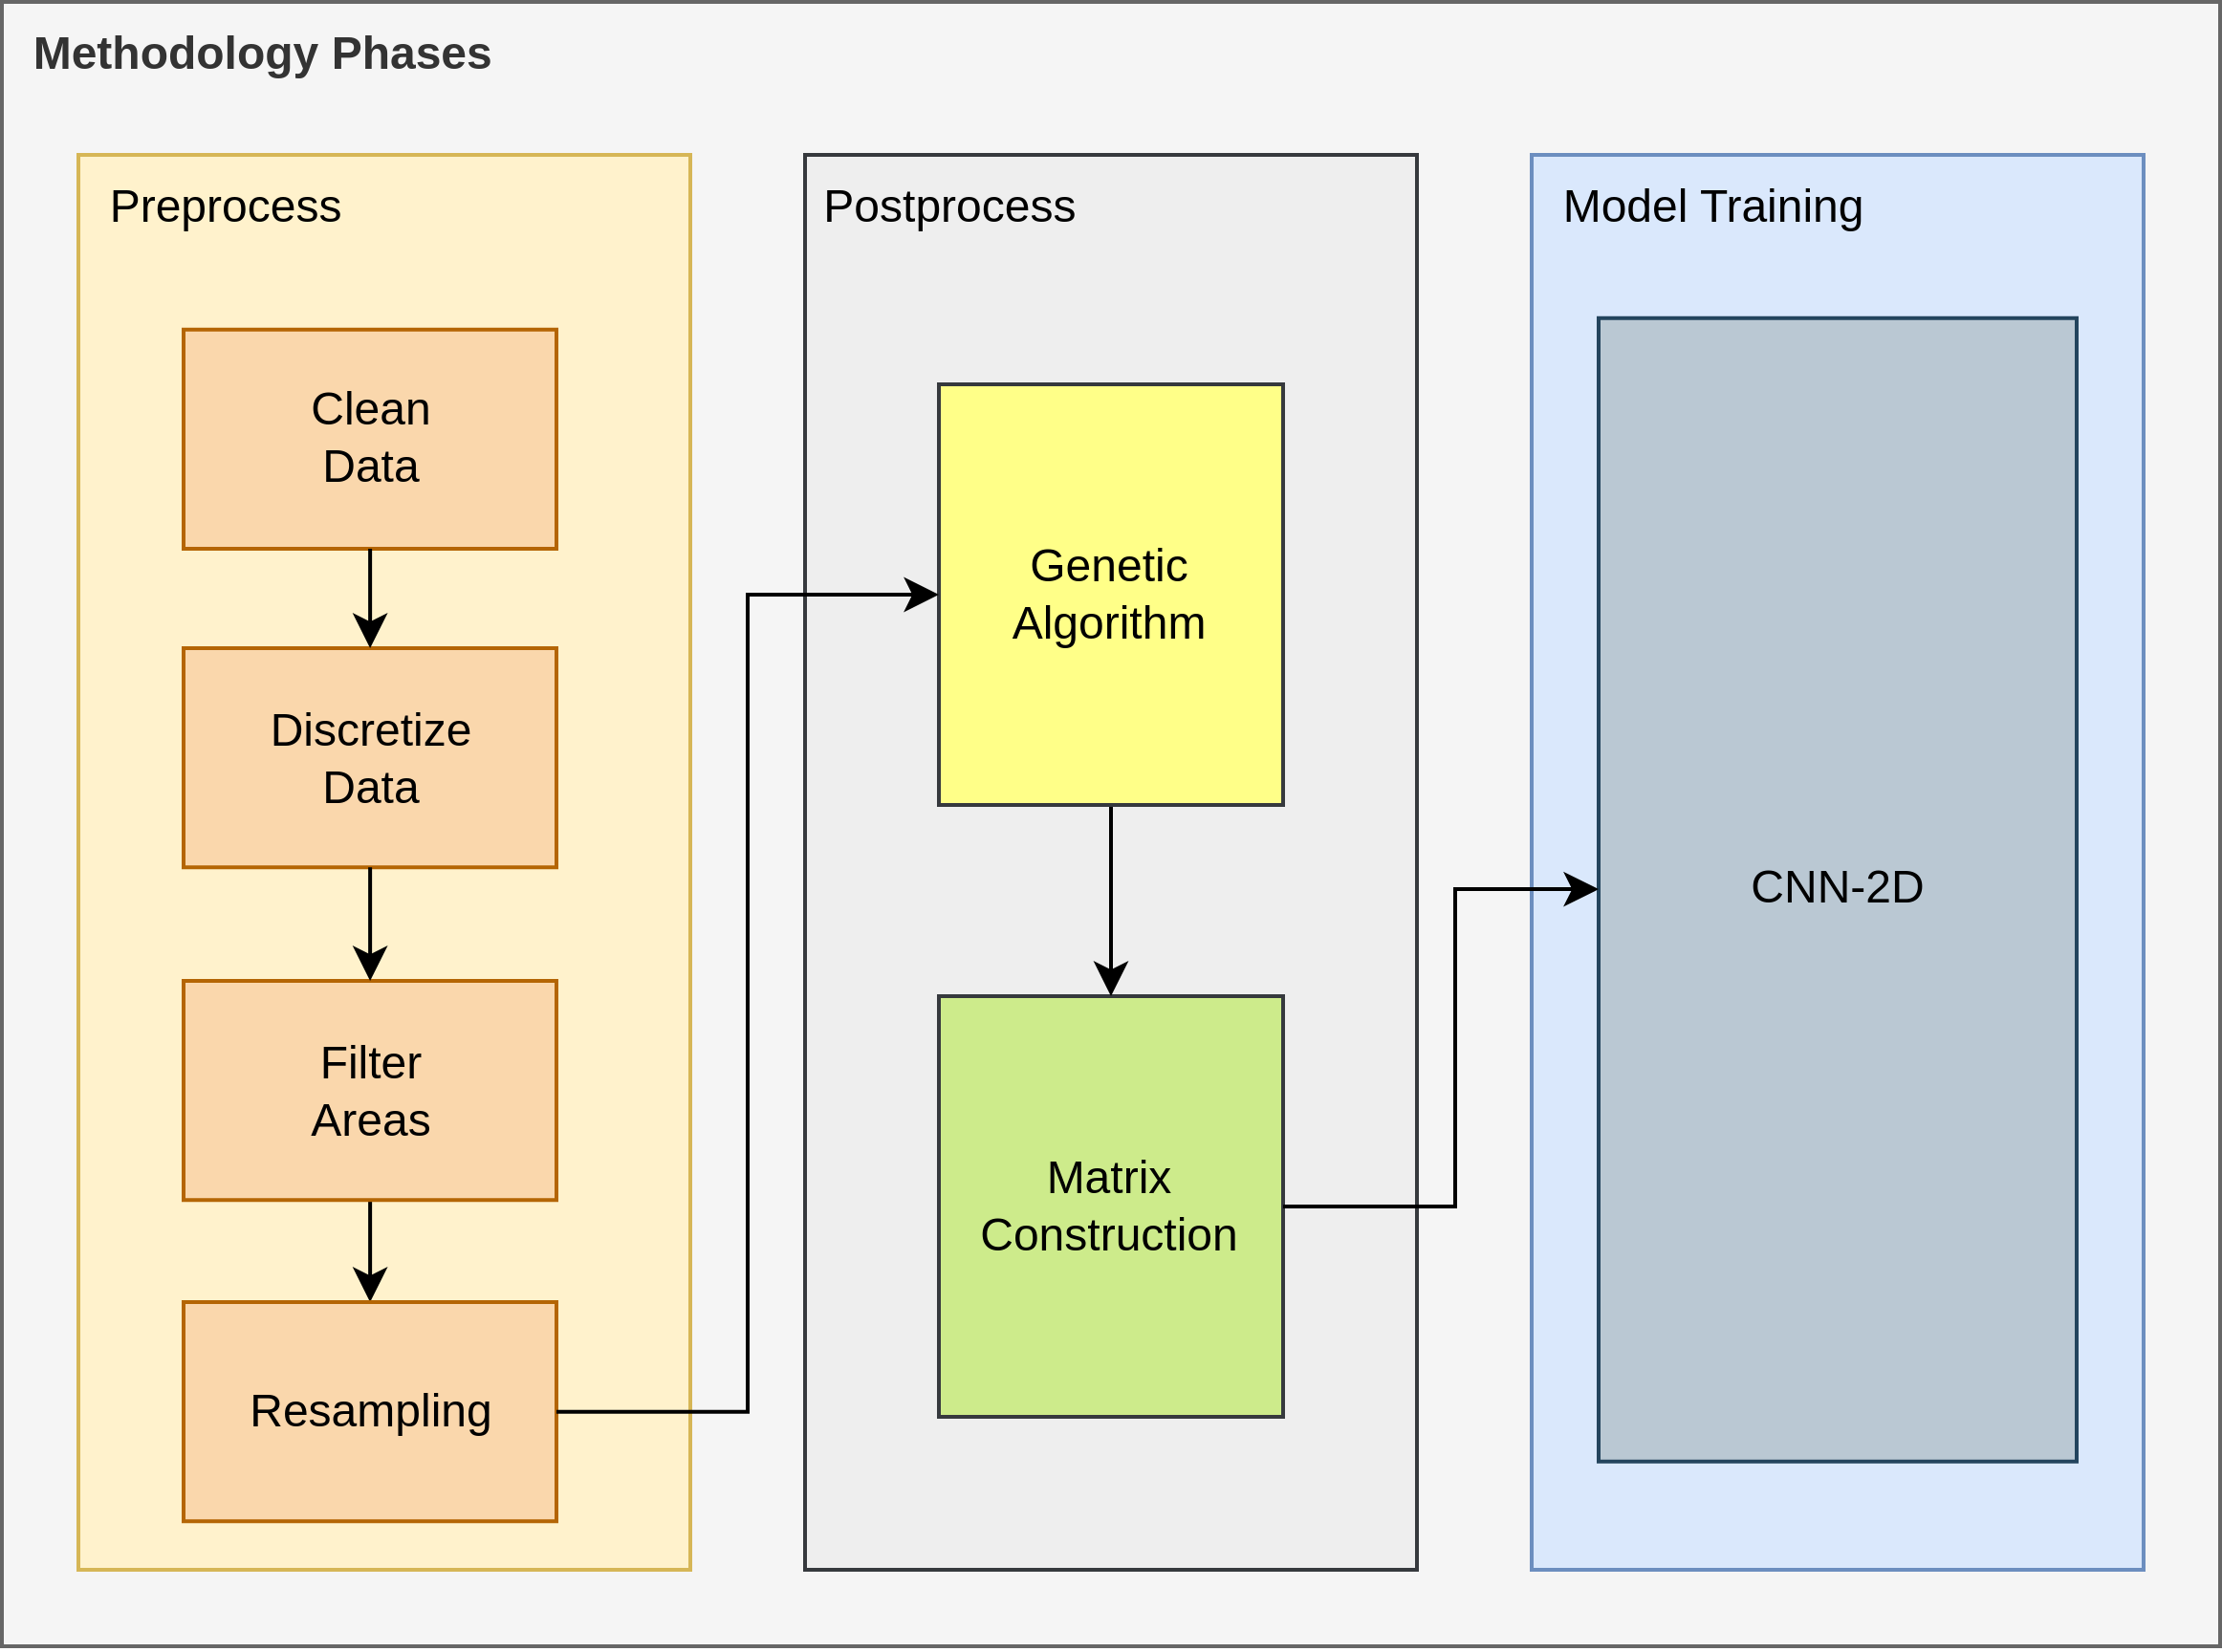
\includegraphics[width=12cm]{Figures/7th DataFlow Chart.png}
	\caption[Diagrama de flujo del modelo GTAAF]{Diagrama de flujo del modelo GTAAF. Consta de tres fases simplificadas: pre-procesado de datos, postprocesado y entrenamiento del modelo}
	\label{DataFlow}
\end{figure}

En segundo lugar, el concepto de gravedad de los accidentes es reasignado de tres a dos clases, accidentes sin necesidad de asistencia y accidentes con necesidad de asistencia. Esto se debe a que el balance entre lo que aporta y lo que resta el distinguir tres clases de accidentes, se decanta claramente por esto último ya que, un modelo de clasificación, a medida que incrementa el número de clases, tiene más posibilidades de realizar predicciones erróneas, sobre todo si son clases minoritarias y existe una clase intermedia conflictiva entre ellas. Por este motivo se distinguen dos clases de accidentes: \textbf{Con Asistencia} y \textbf{Sin Asistencia}.

Como tercera consideración, para paliar aún más el efecto del desbalanceo presente en los datos se diseña una técnica para balancear el dataset en base a la clase minoritaria aplicando un filtrado de áreas. Esta técnica tiene como objetivo dividir el mapa de la población en celdas, para seleccionar aquellas zonas de la región donde existan ambos tipos de accidentes. Con esto se consigue que la información interpretada por los modelos no se vea condicionada por la naturaleza de los mismos.

Para aportar más información, se añaden transformaciones sobre los datos en base a las variables ya existentes. Así, para capturar la naturaleza periódica de la hora del accidente se representó mediante dos componentes cíclicas utilizando funciones seno y coseno. 
%\textcolor{green}{MANU: está el párrafo acabado? Lo digo por la coma sospechosa tras coseno...}

%\textcolor{orange}{\textbf{Luis: } Coma quitada}

% \textcolor{blue}{\textbf{Luis: no dices nada de la categorización en el modelo preeliminar creo, tienes que mencionarlo}}

Como quinta variación a considerar, se redefinen las categorías donde son asignadas las características, pasando de cinco a seis posibles categorías finales. Con este cambio, se busca una reorganización que facilite la asignación de características a conceptos más generales que representan estas categorías. Esto implica que la definición de las matrices que se construyen pasan de tener una posible dimensión de $5\times5$ a $6\times4$, sobre estos conjuntos de datos siempre y cuando se dispongan características para contemplar las nuevas categorías.

Por otra parte, se han centrado los esfuerzo en desarrollar el modelo convolucional de dos dimensiones CNN-2D. Esto se debió al análisis de entrenamiento de los modelos CNN-1D y CNN-2D, optando por descartar el primero debido a la poca capacidad de generalización sobre el conjunto de validación ofrecido por el modelo unidimensional.

Por último, en un intento de evaluar la generalización del modelo propuesto, se ha probado en distintos datasets y áreas, ampliando los conjuntos de datos sobre los que se aplica el modelo. De esta forma, se incluyendo seis regiones de Reino Unido, una de Australia y Madrid. Además, se ampliaron los modelos del estado del arte contra los que comparar el rendimiento, llegando a seis, \textit{SVC, Naive Bayes, Bagging Random Forest, KNN, Regresión Logística} y una red neuronal Perceptrón Multicapa (\textit{MLP}).

\subsection{Pre-procesamiento}

Esta sección explica las diferentes etapas que componen la fase de pre-procesamiento de GTAAF. En esta etapa es donde se les aplica transformaciones a los datos para obtener a un conjunto de datos refinado e interpretable para cualquier modelo que trabaje con datos en formato tabular. 

Esta etapa está compuesta por cuatro fases: (1) proceso de limpieza de datos, donde se identifican, corrigen y se tratan las inconsistencias sobre los datos, (2) la discretización, donde se convierten las variables continuas en variables discretas y se codifican los valores cualitativos de las características, (3) el filtrado de áreas, donde se reduce el desbalanceo de los datos escogiendo subregiones de la ciudad donde se localicen ambos tipos de accidentes, y (4) el remuestreo, donde se se generan muestras sintéticas de la clase minoritaria para disponer de un dataset balanceado. En la Figura \ref{PreprocessingStage} se muestra el flujo sobre el que pasan los datos para cada una de las diferentes fases que componen la etapa de Pre-procesamiento. Esta figura será referenciada en las siguientes subsecciones en la explicación de las fases de Pre-procesamiento.

\begin{figure}[H]
	\centering
	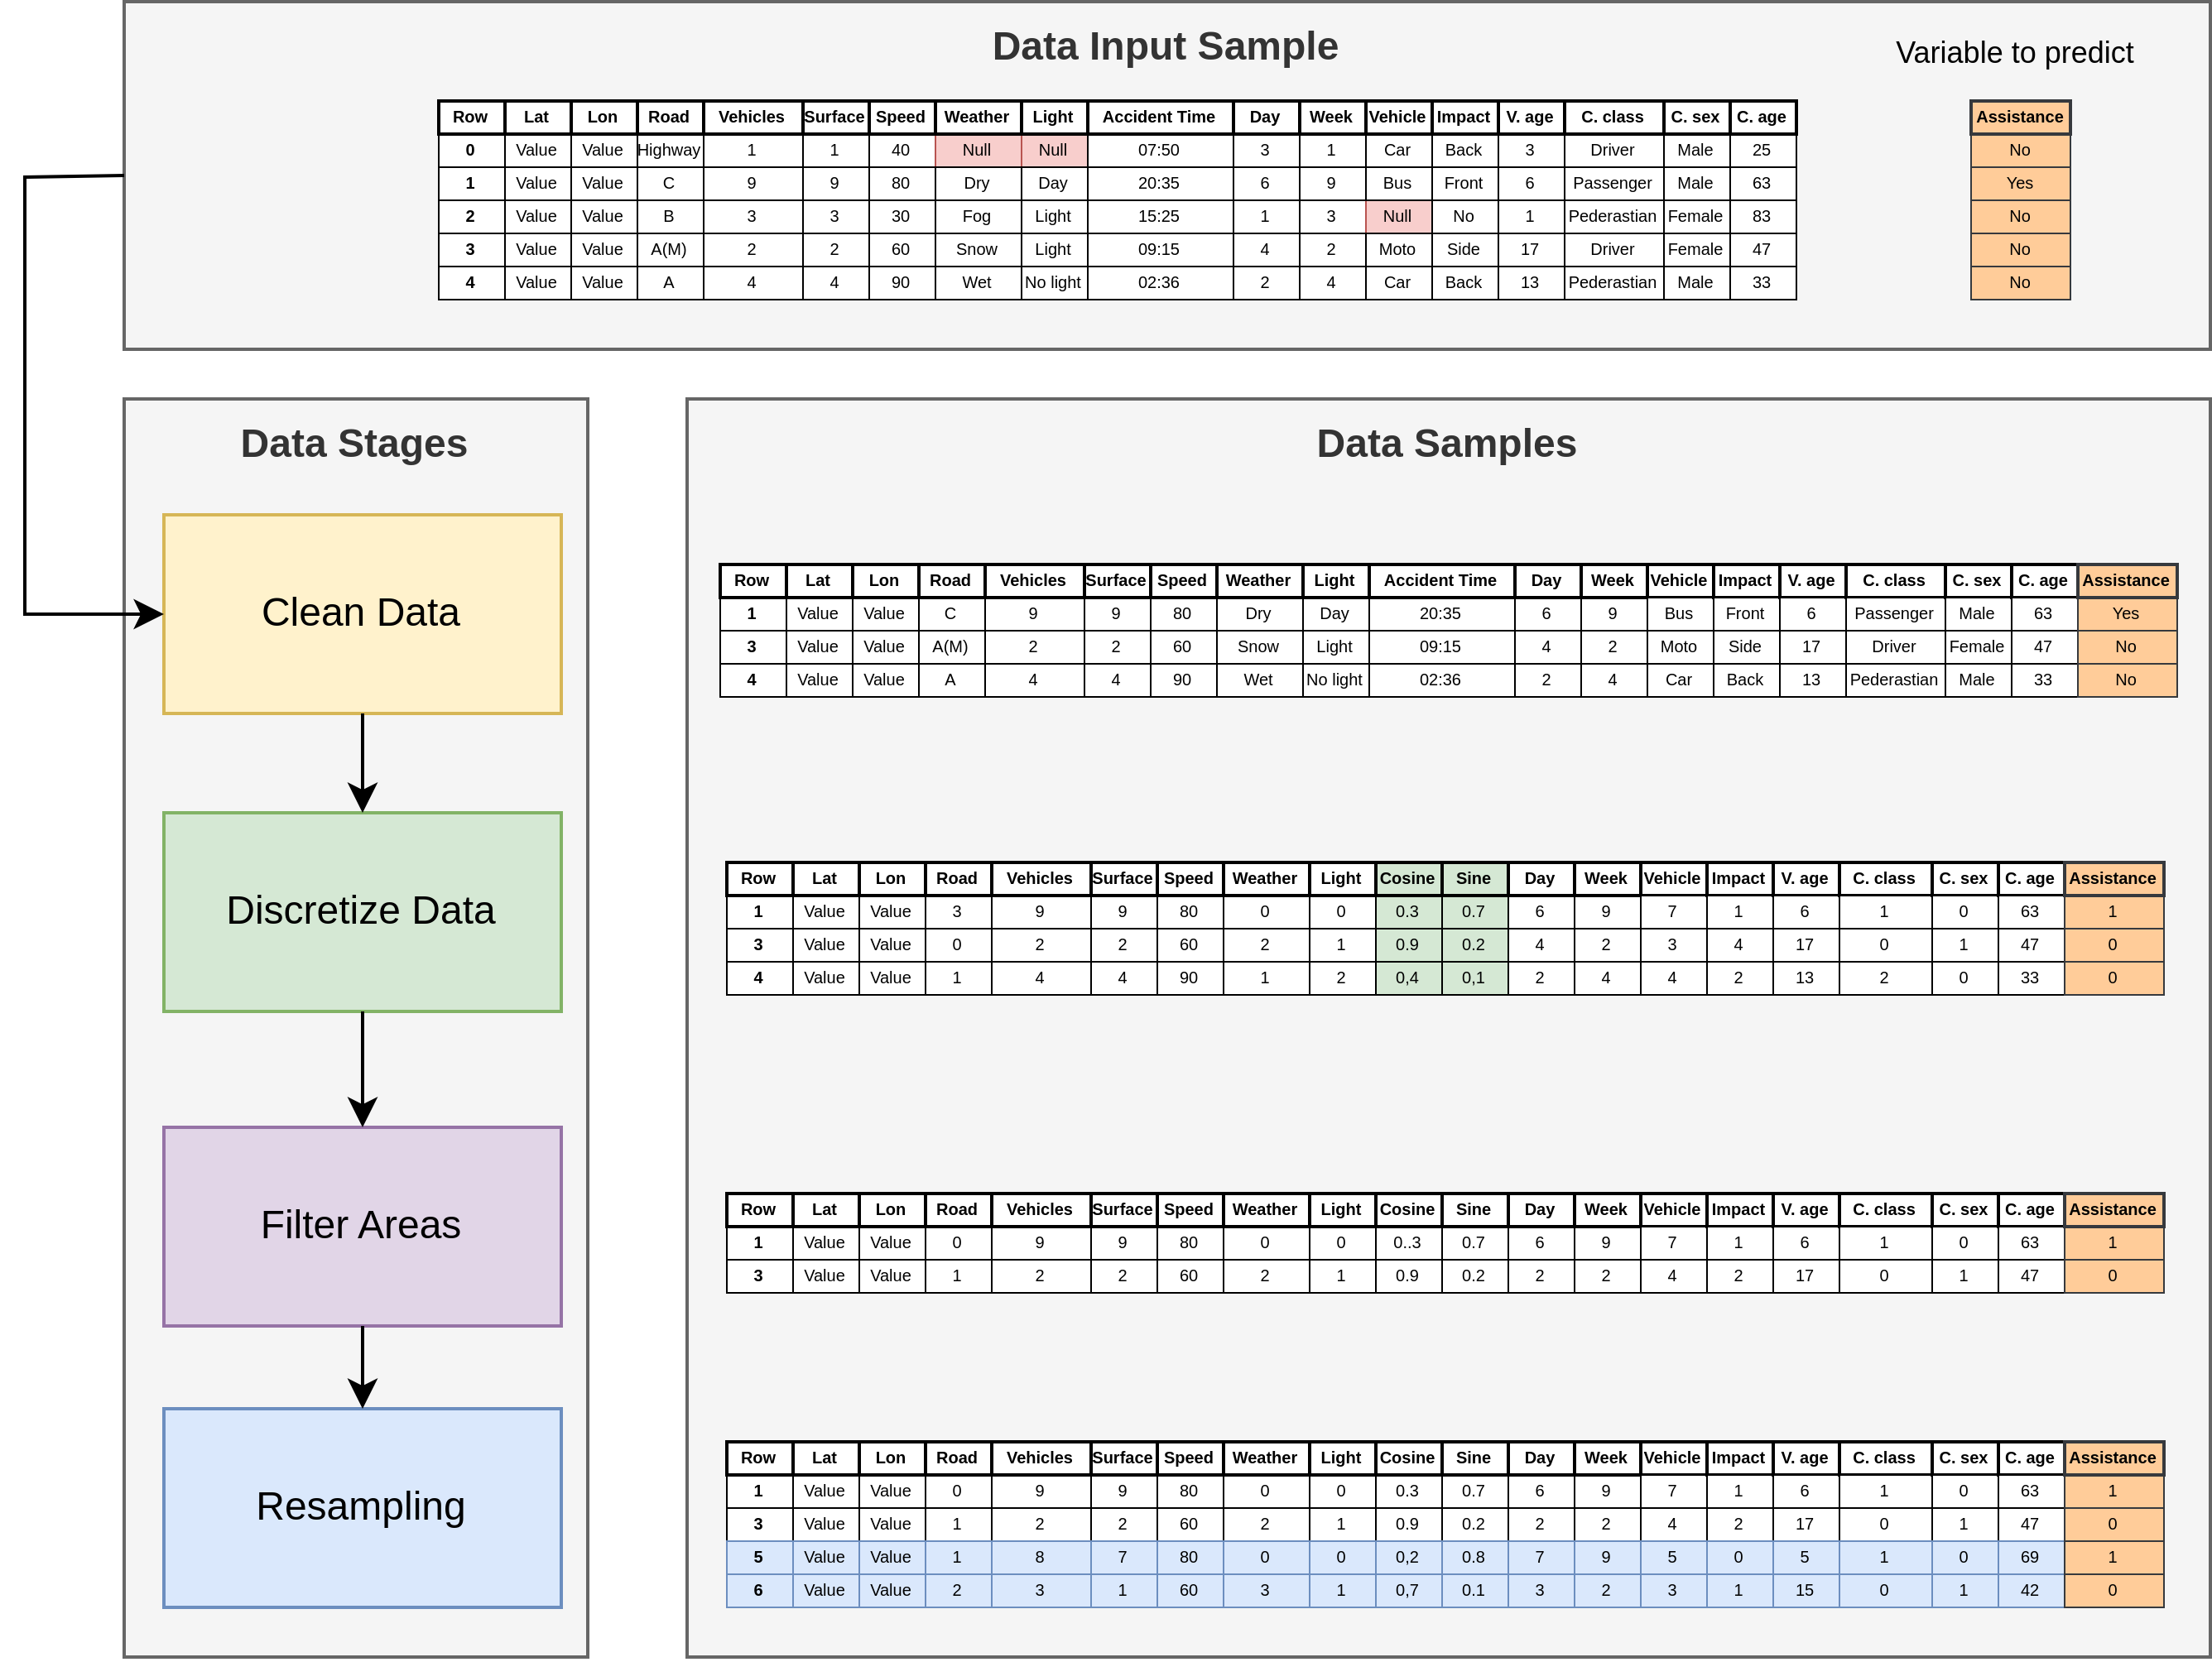
\includegraphics[width=13cm]{Figures/Preprocessing.png}
	\caption[Diagrama de flujo del Preprocesamiento de la modelo  GTAAF] {Diagrama de flujo del Preprocesamiento de la modelo GTAAF. Consta de cuatro fases: (1) limpieza, (2) discretización, (3) filtrado de áreas y (4) \textit{resampling}}
	\label{PreprocessingStage}
\end{figure}

\subsubsection{Limpieza}

La limpieza de datos es un proceso esencial en cualquier proyecto de análisis de datos o inteligencia artificial. Esta fase tiene como objetivo tratar los datos de tal forma que el dataset procesado no disponga de valores ausentes, atípicos, presenten inconsistencias o errores. Este proceso asegura que los datos estén listos para análisis y modelado. Un conjunto de datos limpio y refinado es la base para comenzar a trabajar con modelos predictivos, ya que de otra forma los datos pueden no llegar a ser fiables debido a la incertidumbre presente en ellos \cite{ilyas2019data}.

La primera fase del modelo contempla un proceso de limpieza, en el que aquellos registros de los datos que presenten valores nulos o aquellos que se muestren atípicos sobre las variables escogidas serán eliminados del dataset. Esto provoca que haya un porcentaje de los datos que son eliminados. Estos casos se encuentran representados de color rojo en la primera etapa de la figura \ref{PreprocessingStage}-naranja, donde los registros de accidentes con identificador $0$ y $2$ son eliminados del conjunto de datos al presentar valores vacíos en alguna de las características de interés seleccionadas.


\subsubsection{Discretización}

Los modelos predictivos trabajan con datos numéricos, que son los que están diseñados para interpretar, sobre los que realizan operaciones matemáticas para adquirir conocimiento y poder realizar inferencias sobre muestras nunca antes vistas. Es por esto que las características ofrecidas en los conjuntos de datos deben ser transformadas a estos valores sin perder el utilidad que representa la información. A la hora de describir un accidente, gran parte de la información que se obtiene tiene una naturaleza cualitativa y/o descriptiva. Esto se puede intuir de forma clara con el ejemplo de una característica que describa el punto de impacto del accidente, donde los valores que esta variable pudiera tomar se refiriesen a una descripción cualitativa del punto de impacto del vehículo, como pudieran ser: frontal, lateral o por alcance, entre otras. Por este motivo es necesario aplicar un proceso de cuantificación y discretización que busque transformar estos valores descriptivos en valores numéricos, de tal forma que los datos puedan ser interpretados por los modelos. Se busca representar de forma jerárquica la importancia de cada uno de los posibles valores descriptivos asignando un valor numérico que contemple la importancia ascendente de cada descripción, teniendo como objetivo que la información descriptiva contenida sea coherente con su representación numérica.

% Por este motivo, en esta sección se expondrán el proceso que se ha seguido para transformar las variables cualitativas a cuantitativas, realizando una propuesta de cuantificación en la que se asigna un valor numérico a cada variable en función de la importancia dentro del total de valores que cada una de estas puede contener.

En este trabajo se ha seguido un procedimiento de discretización incremental, donde a cada posible valor del conjunto de datos se le ha asignado un valor numérico en función de la importancia que se le ha asignado, véase \ref{PreprocessingStage}-verde.

%\textcolor{green}{MANU: corregidme si me equivoco, pero en este apartado dijimos que no deberían salir nombre de caracteristicas como aparecen en los datasets, sino mas genérico tipo 'donde los valores que esta variable pudiera tomar se referirían a una descripción cualitativa del punto de impacto del vehículo, como podrían ser frontal o lateral, por ejemplo.'}

%\textcolor{orange}{Luis: había puesto los valores, lo cambiado}

\subsubsection{Transformación (Sin/Cos)}

%\textcolor{blue}{\textbf{Luis: esto yo creo que estaría, a la espera de poner más bonito el dibujo.}}\\

Como se ha comentado anteriormente, los modelos de inteligencia artificial y aprendizaje estadístico interpretan los datos en forma numérica. El valor numérico que se le asigna a cada campo es crítico, ya que será así como el modelo interprete el orden de los valores cualitativos que los humanos somos capaces de comprender. La representación del formato de la horas y minutos del día, por su naturaleza, no es una excepción. El concepto de la hora del día tiene un componente cíclico que es necesario representar para que el modelo comprenda que las 11:59 de la noche es una hora muy próximas a las 00:00. Esto es algo a lo que los seres humanos estamos acostumbrados, pero debe ser indicado de forma coherente para los modelos de inteligencia artificial que interpretarían que estas dos horas muy parejas son valores totalmente opuestos en el rango numérico que puede contener la característica con el formato 24 horas que conocemos. Con el objetivo de representar de forma consistente la información de la hora del accidente, es necesario aplicar una transformación que interprete las horas y minutos en formato 24h a un formato cíclico, y para ello se transformará este campo inicialmente de una dimensión, a dos dimensiones sinusoidales. Para realizar este proceso en primer lugar se transforma la hora y el minuto en el que se ha producido cada accidente a segundos. Posteriormente se aplican las siguientes fórmulas sobre los segundos para representar la hora del accidente en dos componentes, el senosoidal y el cosenoidal (ecuaciones \ref{SIN_EQUATION} y \ref{COS_EQUATION} respectivamente).


\begin{equation}
	\sin((2 \cdot \pi \cdot DaySeconds)/SecondsInDay)
	\label{SIN_EQUATION}
\end{equation}
\begin{equation}
	\cos((2 \cdot \pi \cdot DaySeconds)/SecondsInDay)
	\label{COS_EQUATION}
\end{equation}

%(Dibujito explicativo de senos y cosenos)[puedo poner las 23:59 de la noche representada en seno y coseno, las 00:00 y las 15:00 para que se vean las diferencias].

En la figura \ref{HoursPlot} se muestra un ejemplo de la naturaleza cíclica de la representación de la variable Hora en forma de seno (eje de ordenadas) y coseno (eje de coordenadas), donde se observa que la hora 22:20 en el espacio bidimensional se encuentra más cercana a la hora 01:45 respecto a cualquier otra posible representación unidimensional.

\begin{figure}[h]
	\centering
	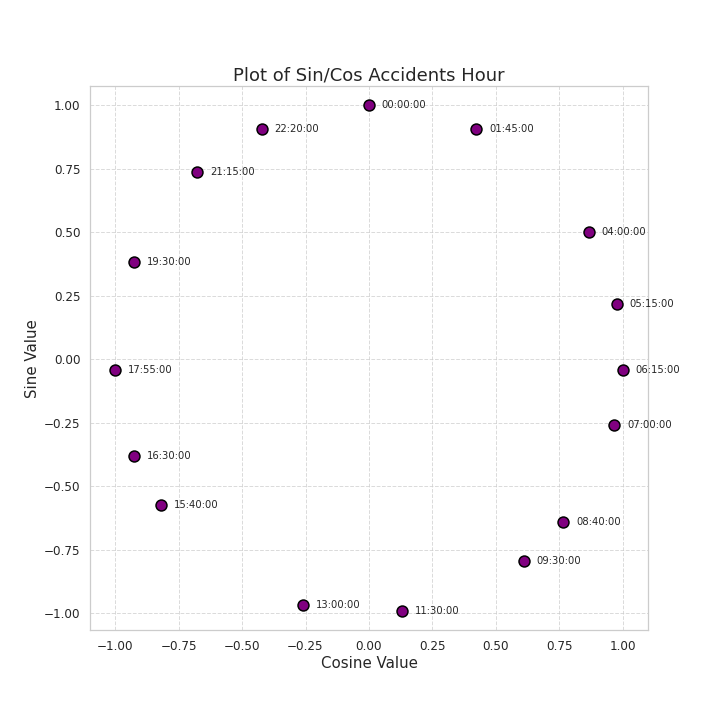
\includegraphics[width=10cm]{Figures/normal_plot.png}
	\caption{Representación de las horas en formato de seno y coseno}
	\label{HoursPlot}
\end{figure}

Esta transformación sobre los datos puede apreciarse en el diagrama de flujo de Preprocesado \ref{PreprocessingStage}-verde, donde se incluyen las nuevas componentes temporales y se elimina la hora del accidente.

\subsubsection{Filtrado de Áreas}

Uno de los retos más comunes en el campo de la inteligencia artificial es disponer de un conjunto de datos no balanceado. Este problema implica tener una desproporción del número de muestras en base a la variable a predecir. Esta casuística afecta negativamente al entrenamiento de los modelos, ya que estos en su etapa de entrenamiento adquieren el conocimiento prediciendo sobre estas muestras y son penalizados cuando sus predicciones durante esta fase son erróneas. Si la distribución de datos de entrenamiento dispone de muchas más muestras de una clase que de otra, el modelo tenderá a aprender durante su entrenamiento a predecir siempre aquella clase mayoritaria, ya que se le ha penalizado en menos ocasiones durante esta fase, obteniendo así un modelo sesgado que está condicionado por naturaleza a predecir sobre la clase más común.

En lo que respecta la naturaleza de la distribución de datos de accidentes de tráfico, siempre existirán muchos más accidentes que no han necesitado asistencia respecto a los que sí. Por lo que durante esta fase del modelo se busca paliar este efecto tratando de reducir la diferencia entre el número de registros de la clase mayoritaria (sin necesidad de asistencia) y la clase minoritaria (necesidad de asistencia).

Para solventar esto se aplica un filtrado basado en áreas, que buscará balancear los datos escogiendo áreas estratégicas donde coexistan accidentes con ambos tipos de consecuencias. Para cada población se establece una ventana de dimensiones (\textit{X,Y}) que recorrerá secuencialmente el área total que engloba cada una de las regiones escogidas en esta tesis. Esta ventana buscará si en ese área coexisten accidentes de tipo No-Asistencia y Asistencia, de tal forma que si esto se cumple, dicha subárea se mantendrá en el dataset, y en caso contrario se eliminará. Esto consigue un balanceo de los datos que minimiza el número de accidentes de tipo No-Asistencia en el dataset que no sean estrictamente necesarios. En la figura \ref{Areas} se muestra un ejemplo del criterio seguido para aplicar este filtrado, donde se seleccionan únicamente aquellas regiones donde coexisten accidentes sin necesidad de asistencia (verde) y con necesidad de asistencia (rojo).


\begin{figure}[H]
	\centering    
	\subfloat[Ejemplo de muestras de accidentes originales]{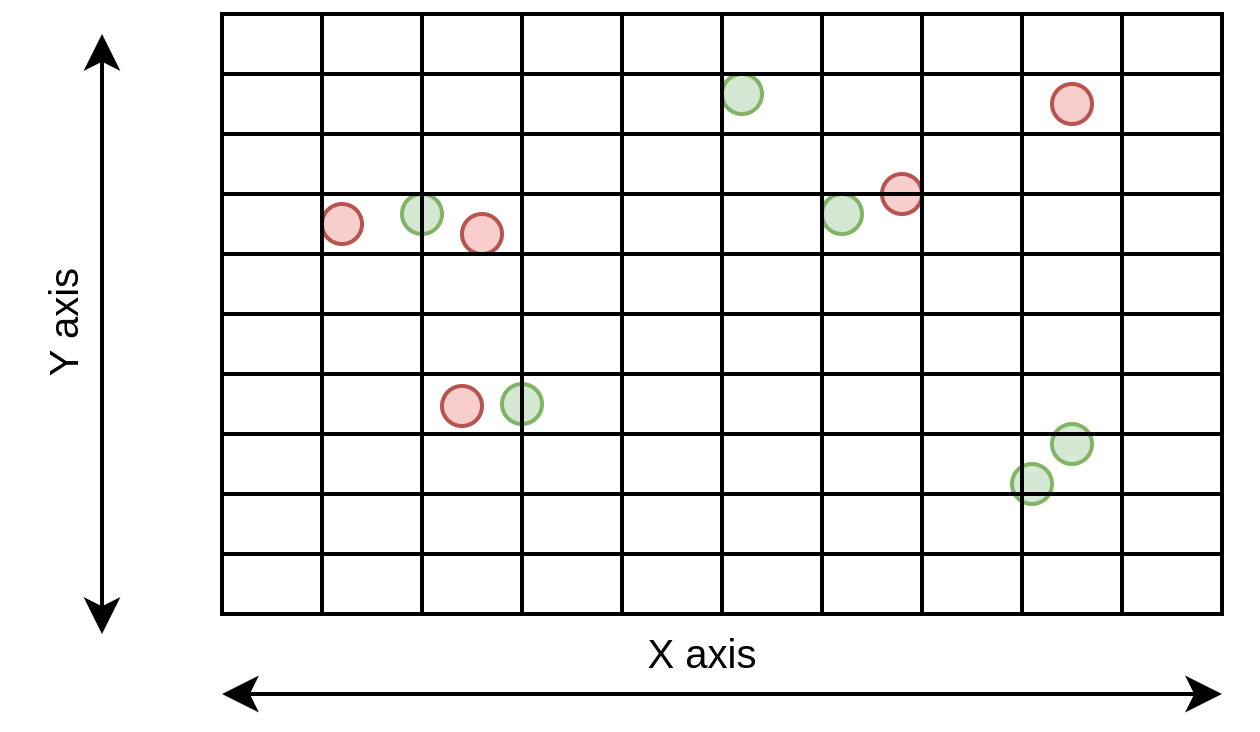
\includegraphics[width=6cm]{Figures/areas-points.png}}
	\subfloat[Ejemplo de muestras de accidentes filtradas]{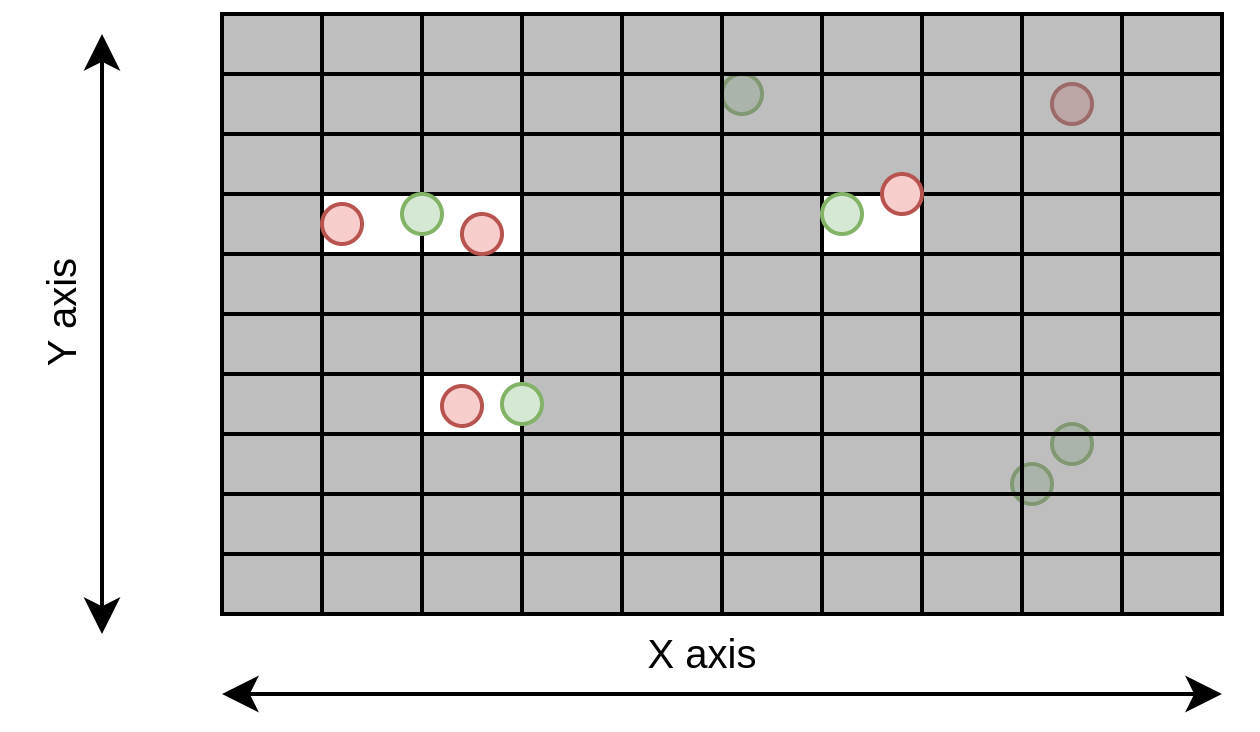
\includegraphics[width=6cm]{Figures/areas-points-filtered.png}}
	\caption[Ejemplo de filtrado de áreas]{Ejemplo de filtrado de áreas. Los puntos verdes representan accidentes que no requieren asistencia, mientras que los puntos rojos representan accidentes que necesitan asistencia}
	\label{Areas}
\end{figure}

En la Figura \ref{PreprocessingStage}-morado se muestra el ejemplo donde el accidente sin necesidad de asistencia con identificador $4$ se elimina del conjunto de datos porque no convive con otro accidente de tipo asistencia dentro de su mismo área.

\subsubsection{División de datos}

%\textcolor{blue}{\textbf{Luis: esto yo creo que estaría, lo único hacer inciso en lo último.}}\\

Los modelos supervisados de inteligencia artificial aprenden patrones sobre datos que son ofrecidos en la etapa de entrenamiento del modelo. Durante esta fase los modelos realizan predicciones sobre de datos y posteriormente se les enseña la clase a la que pertenecía cada uno de los datos que ha predicho, de esta forma se mide el error que han cometido durante este proceso y los pesos de la red son actualizados para minimizar el error en la siguiente fase. Si este aprendizaje se repite durante muchas etapas, el modelo tiende a aprender los datos de memoria, lo que se conoce como sobreajuste de la red u \textit{overtfitting}, provocando que la red no sea capaz de generalizar ante nuevas muestras tras su entrenamiento. Por este motivo es importante mantener el control del aprendizaje de la red mediante la evaluación de su rendimiento en cada época de entrenamiento mediante un conjunto de datos que nunca ha visto durante su fase de aprendizaje, este conjunto de datos es conocido como conjunto de validación, y es utilizado como referencia para limitar el entrenamiento cuando el modelo no sea capaz de generalizar sobre estas nuevas muestras. Por otra parte, existe un conjunto de datos de test, utilizado para medir el rendimiento del modelo final una vez ha acabado su fase de aprendizaje. Este conjunto pertenece a muestras que la red no ha visto durante su fase de aprendizaje ni ha sido utilizado como validación.

En este trabajo se ha dividido el conjunto de datos original de cada una de las ciudades mediante el porcentaje $80\%$ para entrenamiento y $20\%$ para validación y test.


\subsubsection{Resampling}

Una vez se disponen de los datos refinados, es necesario aplicar algún proceso que logre balancear los datos en función de la clase a la que pertenecen. El conjunto de datos, una vez se han reducido considerablemente el desbalanceo entre las dos clases gracias al proceso de filtrado de áreas, sigue presentando cierto desbalanceo. Por mucho que se haya acotado el problema a regiones individuales, es lógico que se hayan producido más accidentes sin necesidad de asistencia respecto a los que sí la requieren.

En el caso de estudio de esta tesis, aplicar técnicas de \textit{Undersampling} que eliminen accidentes sin necesidad de asistencia hasta igualar el número de aquellos que sí la requieren es un inconveniente, ya que al disponer de tan pocas muestras de la segunda clase, el conjunto de datos resultante se vería notablemente reducido y afectaría negativamente al entrenamiento de la red que requiere de un conjunto de datos lo más extenso posible para favorecer la generalización en sus predicciones.

Por este motivo, se opta por métodos de aumentado de datos (\textit{Upsampling}), que mantienen el valor que aportan las muestras de los accidentes sin necesidad de asistencia, aumentando los datos de aquellos que sí la requieren. Se ha optado por una técnica de generación de datos sintética denominada \textit{Synthetic Minority Oversampling Technique (SMOTE-II)}, que busca incrementar el número de clases de las muestras minoritarias mediante la generación de nuevas muestras artificiales.

En la Figura \ref{PreprocessingStage}-azul se observan, marcados en azul, cómo los registros con identificadores $5$ y $6$ han sido generados en base a las modificaciones de los valores de los registros $1$ y $3$ para balancear el dataset.



\subsubsection{Normalización}

En cualquier modelo de inteligencia artificial es imprescindible normalizar los datos. Los modelos predictivos trabajan con valores numéricos realizando operaciones sobre ellos. En los conjuntos de datos suelen coexistir variables cuyos valores se encuentran representados en distintas escalas, es decir, que los valores que pueden tomar ciertas características suelen presentar un rango de valores mucho más amplio que otras de ellas dentro del mismo conjunto de datos, haciendo que las características sean incomparables entre sí debido a la diferencia entre su magnitud. Un ejemplo de esto puede observarse en una característica que pudiera describir la semana dentro del año en el que se ha producido el accidente y, por otra parte, el sexo de la víctima. La primera de estas variables puede contener un amplio rango de posibles valores (desde el $0$ hasta el $51$), en función de la semana en la que se ha producido el accidente, mientras que la segunda variable únicamente puede tomar dos valores ($0$ ó $1$). Esta diferencia numérica en los posibles valores de los datos provoca que las operaciones matemáticas que aplican los modelos durante su fase de entrenamiento sean desproporcionadas en las características con rango de valores más altos, produciendo una desproporción en estas operaciones y provocando que los datos incomparables entre sí, dándole más importancia a unas características que a otras. Es por esto por lo que es necesario un proceso de logre acotar el rango de posibles valores del conjunto total de datos para poder operar sobre todos los descriptores con la misma importancia. Existen distintas técnicas para aplicar la normalización en los datos, como \textit{Mean Centered (MC)}, \textit{Variable Stability Scaling (VSS)} o \textit{Min-Max Normalization (MMN)}, entre otras \cite{DataNormalizationInvestigation}. En este trabajo para normalizar los datos y hacerlos comparables entre sí se ha utilizado la técnica de \textit{Z-Score (ZSN)} (ecuación \ref{Z_SCORE_EQUATION}) debido a que logra representaciones de acuerdo con una distribución normal. Para hacerlo, se utilizan la media y la desviación estándar para reescalar los datos de manera que su distribución esté definida por una media de cero y una desviación estándar unitaria.

\begin{equation}
	\label{Z_SCORE_EQUATION}
	Z = \frac{(X - \mu)}{\sigma}
\end{equation}




\subsection{Post-procesamiento}

La segunda fase del modelo GTAAF implica transformar los datos refinados y balanceados en matrices interpretables por el modelo GTAAF propuesto. Este proceso conlleva asignar los atributos de las muestras tabulares en posiciones dentro de estas matrices. Para realizar esto, se hace uso de un método de transformación que toma en consideración la importancia de cada característica dentro del conjunto de datos. El objetivo es posicionar estratégicamente las características más relevantes en la matriz para maximizar su impacto en el modelo GTAAF, como se ilustra en la Figura \ref{PostprocessingStage}. La determinación de la importancia de las características se basa en un algoritmo tipo boosting, \textit{XGBoost}, que asigna pesos a las variables según su relevancia en la separación de datos durante el entrenamiento de este. Para garantizar un entrenamiento óptimo del modelo, se realiza una optimización de hiperparámetros utilizando algoritmos evolutivos. A lo largo de generaciones sucesivas, este algoritmo genético hace evolucionar los hiperparámetros, guiado por la métrica de \textit{F1-Score}, que actúa como función heurística a optimizar.

\begin{figure}[H]
	\centering
	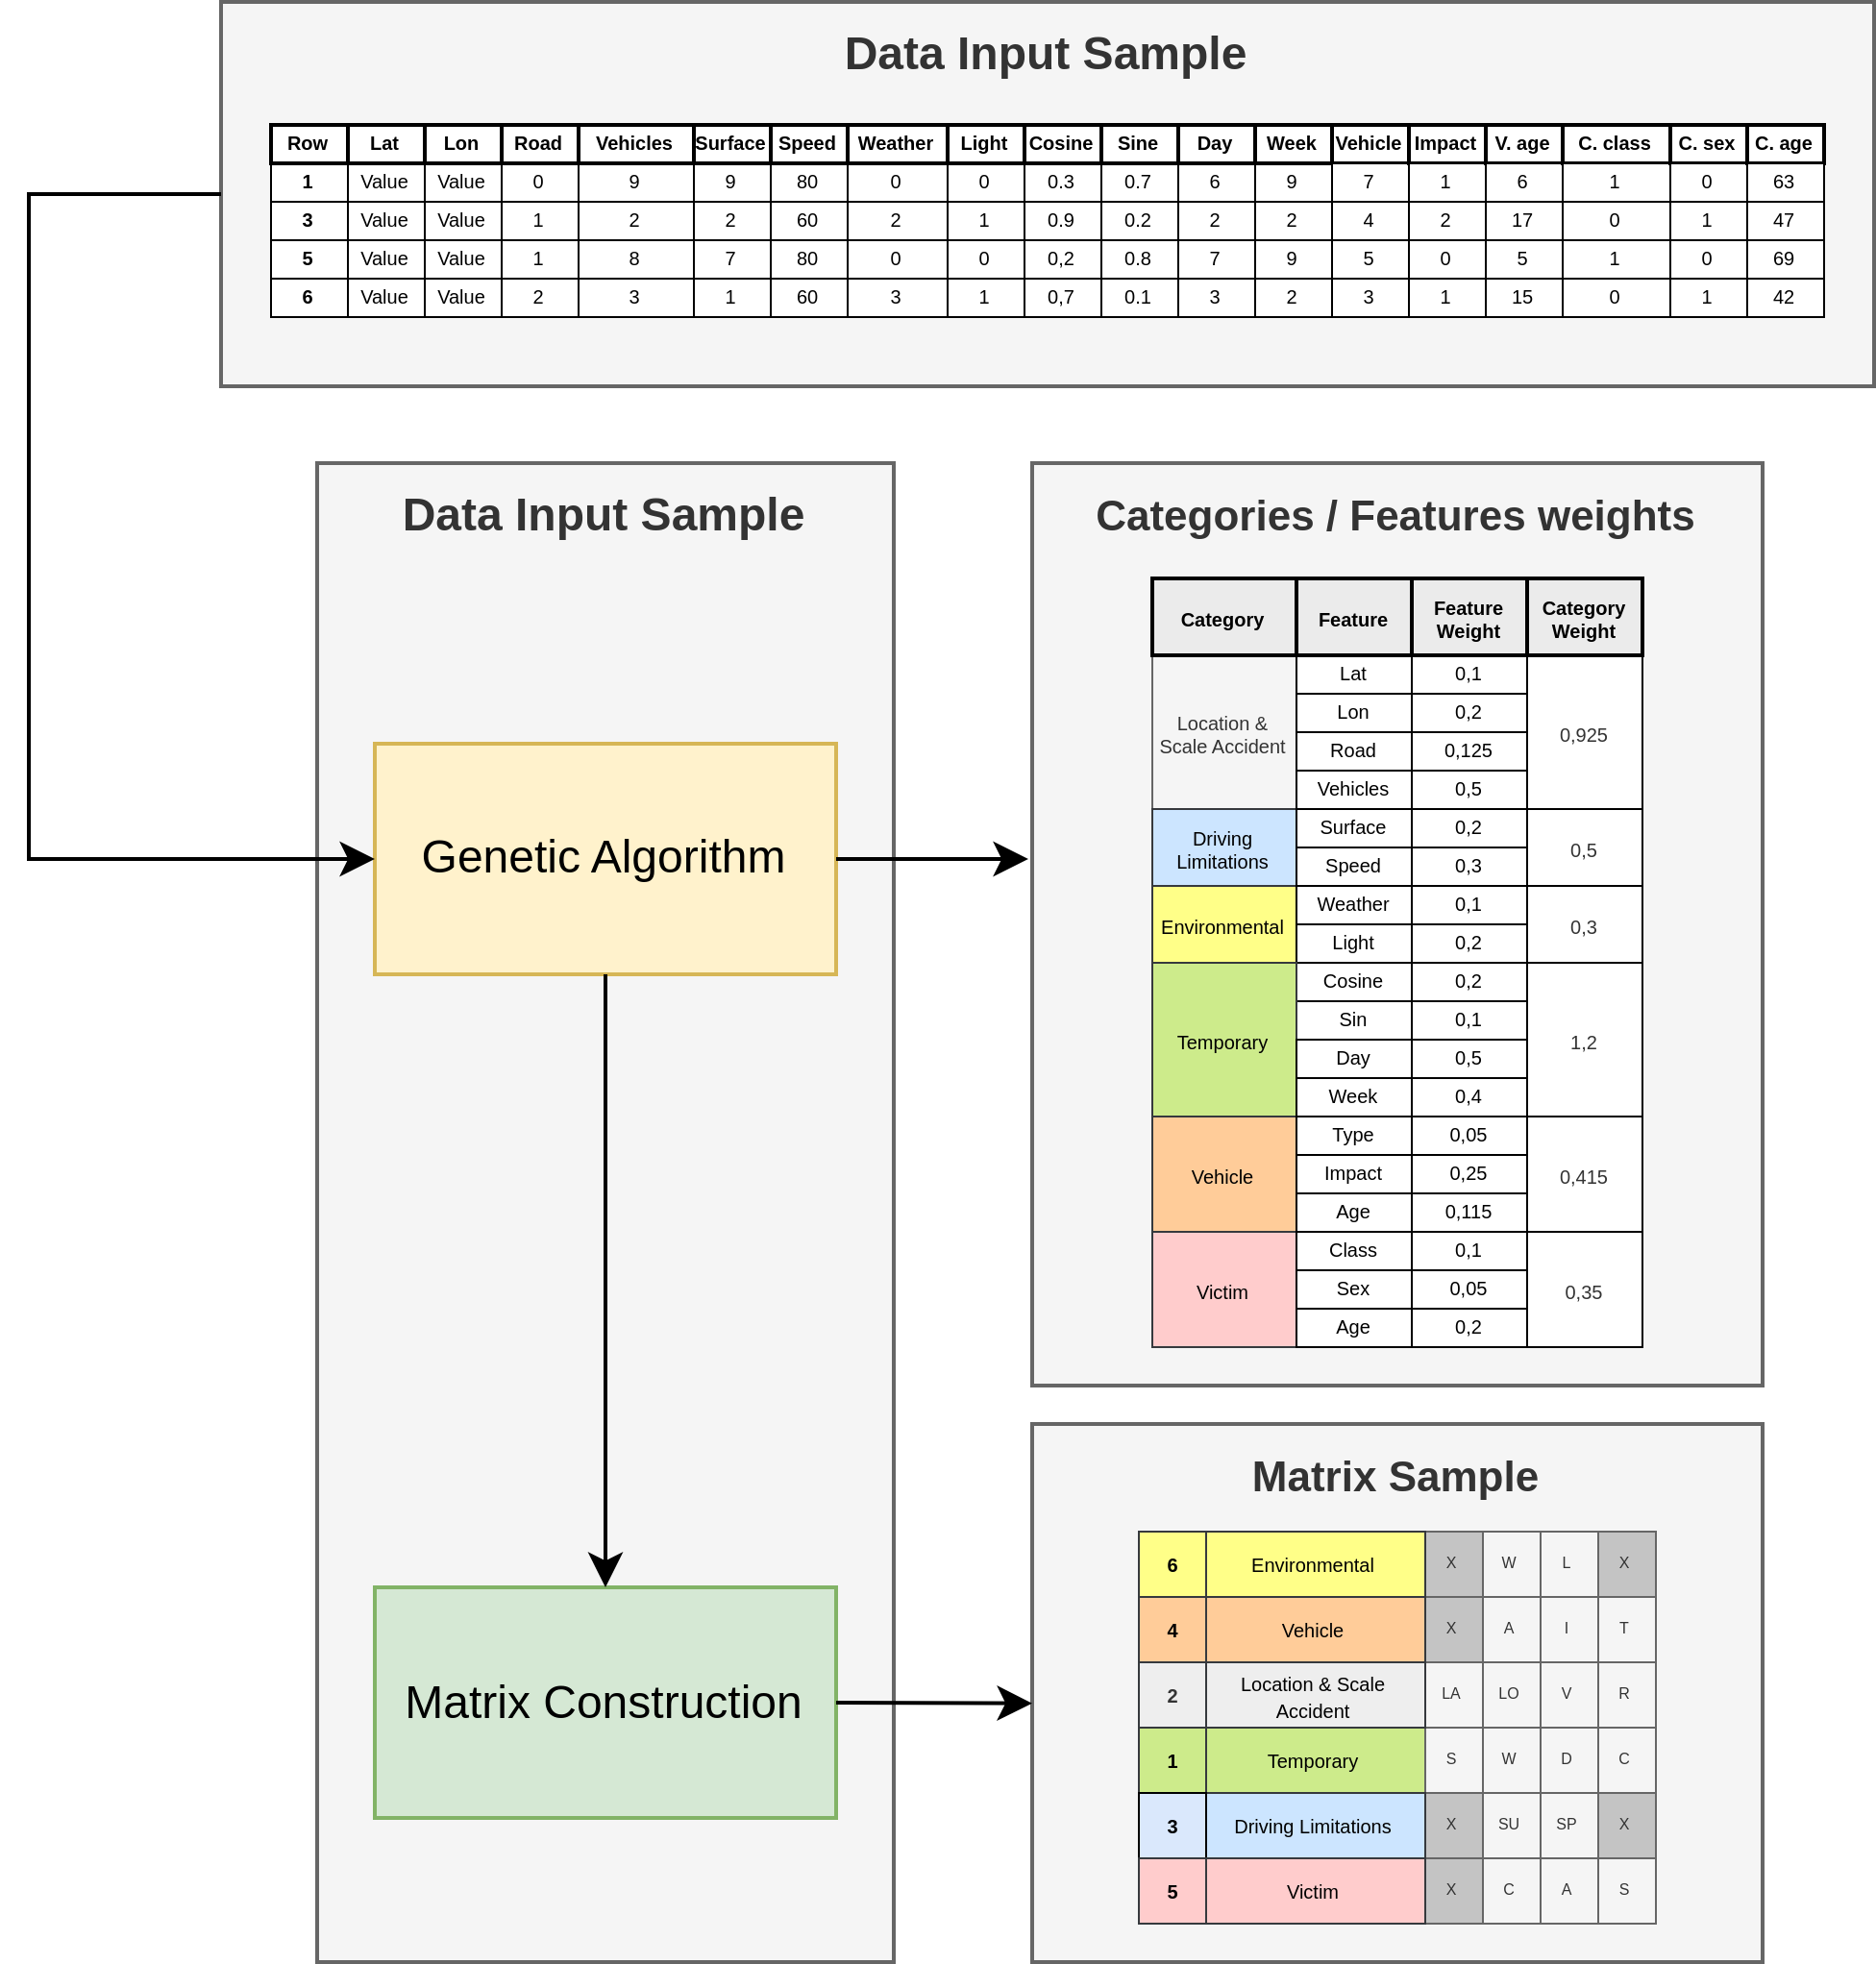
\includegraphics[width=13cm]{Figures/Postprocessing_2.png}
	\caption[Diagrama de flujo del Postprocesamiento de la modelo GTAAF]{Diagrama de flujo del Postprocesamiento de la modelo GTAAF. Consta de dos fases: (1) aplicación del algoritmo genético para la optimización de hiperparámetros de \textit{XGBoost}, y (2) construcción de matrices en base a los pesos de las categorías}
	\label{PostprocessingStage}
\end{figure}

\subsubsection{Construcción de Matrices}

En este trabajo, se presenta un método para transformar datos, inicialmente tabulares, a datos matriciales con los que podrá trabajar el modelo GTAAF. Esta transformación hace uso de la categorización de las características y la importancia de cada una de ellas individualmente dentro del conjunto de datos a las que pertenecen. En secciones anteriores se ha explicado el funcionamiento del proceso de categorización propuesto, que busca poder aplicar este modelo a cualquier conjunto de datos de accidentes, agrupando las características en conceptos básicos y de fácil obtención. El siguiente paso para lograr la transformación de los datos, inicialmente en filas y columnas, a datos matriciales es asignar cada una de las características del conjunto de datos a una posición dentro de la matriz, de tal forma que los datos puedan ser interpretados por el modelo convolucional. Para tener un contexto de la importancia en el orden en el que se asignan estas características, se explica brevemente la intuición sobre la que trabajan las redes neuronales convolucionales. Los píxeles que componen una imagen representan patrones que, para los seres humanos, son reconocibles, las redes convolucionales aprenden a reconocer estas variaciones inicialmente en una escala pequeña (pocos píxeles) y, a medida que aumenta el número de capas de las que se componen estas redes son capaces de aprender patrones más complejos en base a la composición de aquellos más simples. Este funcionamiento, por definición, implica que la forma en la que se construye una imagen artificial sea crítica, es decir, que el contenido que representa la imagen debe estar formado de manera coherente para que las redes puedan aprender estos patrones, requiriendo un sentido y/o contexto completo en su composición.

Existen distintos métodos que logran transformar datos tabulares a una representación matricial de los mismos, buscando dar un sentido a la asignación de las características en posiciones de la matriz. En la sección \ref{SOAT_MATRIX_ALGORITHM_CONSTRUCTION} se presentaron distintos métodos como \textit{REFINED, DeepInsight} o \textit{IGTD}, que buscan optimizar la posición de las características en base a la similaridad que presenten entre ellas, principalmente en datos orientados a la descripción genética. Sin embargo, estas técnicas presentan distintas limitaciones debido a la magnitud de los datos para las que han sido diseñadas (del orden de $2500$ características), esto provoca que estos métodos sean difícilmente aplicables a datos de baja dimensionalidad, pudiendo asignar espacios en blanco ante la falta de características o que los métodos no sean capaces de converger al trabajar con tan pocos datos. En el caso de estudio de esta tesis las características disponibles son mucho menores, del orden de $20$ variables.

Debido a las limitaciones de los métodos anteriores, en este trabajo se presenta un método de composición de matrices en base a la importancia de las características, que permite asignar cada una de las variables del dataset a posiciones estratégicas dentro de la matriz haciendo uso de dos conceptos fundamentales: los algoritmos genéticos y los algoritmos de medición de importancia de características.

\subsubsection{Algoritmos de medición de importancia de características}
%\subsubsection{Feature Importance Algorithm}
\label{FEATURE_IMPORTANCE:ALGORITM_JUSTIFICATION}
%\textcolor{blue}{\textbf{Luis: Floja la justificación, pero van por ahí los tiros.}}\\

Como se ha presentado en la sección \ref{SOAT_FEATURE_IMPORTANCE_METHODS}, existen distintos métodos que permiten evaluar la importancia de las variables en función de distintos criterios, como la correlación que presentan las variables entre sí o el nivel de importancia de cada característica a la hora de entrenar un modelo predictivo. Ejemplos como estos son la Regresión Logística, técnicas de \textit{ensembles} de tipo \textit{Bagging} como los \textit{Random Forest} o métodos \textit{ensembles} tipo \textit{Boosting}.

En esta tesis se trabaja con conjunto de datos desbalanceados, por lo que a la hora de aplicar algoritmos de medición de características es importante escoger técnicas que sean insensibles a esto. Una de las muchas propiedades que ofrecen de los métodos de \textit{ensembles} es que se adaptan especialmente bien a conjuntos de datos sesgados. Estos modelos, en sus distintas formas, se benefician de estar compuestos de una combinación de modelos que, mediante distintas técnicas de muestreo, consiguen reducir considerablemente el sobreajuste que pueda darse con otros métodos.

Dentro de estos modelos, los \textit{ensembles} tipo \textit{Boosting} son ampliamente conocidos por adaptarse especialmente bien en estos casos. Estos modelos utilizan técnicas de regularización durante su entrenamiento y se centran en minimizar el error producido cuando clasifican muestras de aquellas clases más conflictivas, que en el caso de un dataset desbalanceado serían las muestras minoritarias. Por otra parte, son modelos muy robustos que generalmente ofrecen un mayor rendimiento respecto a otros tipos de \textit{ensembles} como los \textit{Random Forest}, que únicamente ofrece que cada uno de los modelos sea entrenado con un subconjunto de los datos originales.

En este modelo se utilizará el algoritmo tipo \textit{Boosting XGBoost}, donde se minimizará el error del modelo mediante la métrica \textit{F1-Score} resultante de la clasificación de ambas clases de accidentes (sin necesidad de asistencia y con necesidad de asistencia).

Este algoritmo ofrece una serie de hiperparámetros, que permiten configurar el método para maximizar su rendimiento. Del total de hiperparámetros disponibles para su configuración, se escogerán aquellos más relevantes, concretamente la profundidad máxima que puede tomar el árbol, el número de árboles que minimizarán el error de sus predecesores y  la tasa de aprendizaje (\textit{learning rate}). Para ello se aplicarán técnicas de optimización de hiperparámetros basadas en algoritmos evolutivos.


% Existen múltiples algoritmos que implementan esta filosofía, entre los que destacan: (1) AdaBoost, orientado a clasificación, que en cada iteración , (2) Random Forest () y (3) XGboost. Para la metodología presentada en esta tesis se ha escogido la técnica XGBoost, ya que las características de este algoritmo son las más adecuadas a este contexto. XGBoost es menos sensible a datos que presentan una alta variabilidad y un importante desbalanceo entre ellos. Además, este algoritmo permite una mejor optimización en sus árboles sucesores al configurar los hiperparámetros con los que se entrena únicamente una única vez para el árbol inicial (profundidad del árbol, número de árboles y learning rate) [2]. El funcionamiento del XGBoost escogido es el siguiente...


\subsubsection{Algoritmo Genético}

Como se ha comentado en la sección \ref{HYPERPARAMETERS_OPTIMIZATION_METHODS}, existen numerosos métodos para optimizar hiperparámetros, cada uno con sus ventajas y desventajas dependiendo del contexto y los datos en el que se apliquen.

Debido a las limitaciones computacionales que supone la combinación de todos los posibles valores de los hiperparámetros, el método \textit{Grid Search} no se adapta adecuadamente al caso de uso contemplado en esta tesis. Por otra parte, siguiendo la línea de probar combinaciones de hiperparámetros sin una evolución en su convergencia, el método \textit{Random Search} aunque ses más eficiente que la búsqueda de cuadrícula, no es idóneo para este caso, ya que no sigue ningún patrón que explote las mejores soluciones que se van obteniendo, siendo estas combinaciones meramente aleatorias.

Debido a esto, en esta tesis se utilizan algoritmos genéticos para optimizar los hiperparámetros de entrenamiento del algoritmo \textit{XGBoost}. Este tipo de algoritmos permiten una exploración amplia del espacio de búsqueda de los hiperparámetros óptimos, acentuando además la explotación en soluciones cercanas al óptimo ideal. El algoritmo con los hiperparámetros optimizados \textit{XGBoost} ofrecerá la importancia de las características, necesaria para la construcción de las matrices de entrada al modelo GTAAF. Donde cada uno de los individuos de la población del algoritmo genético representará una posible combinación de hiperparámetros, concretamente los valores de (\textit{Max Depth}, \textit{ETA} y el número de árboles). La función heurística que será optimizada será el \textit{F1-Score} otorgado sobre los datos de test de cada uno de los conjuntos de datos.

\subsubsection{Construcción de Matrices}

Una vez se dispone de la categorización de los datos y de los pesos de las características gracias al modelo \textit{XGBoost}, se aplica el proceso de asignación de cada una de las variables a posiciones de la matriz. Como se ha comentado en secciones anteriores, la forma en la que se compone una matriz sobre la que opera una red convolucional es de vital importancia y por esto es necesario aplicar un método que logre transformar estos datos de manera coherente y eficiente. Existen diferentes enfoques para construir matrices en base a datos tabulares, pero estos enfoques como se ha comentado en la sección \ref{FEATURE_IMPORTANCE:ALGORITM_JUSTIFICATION} sufren de limitaciones aplicados a nuestro caso de uso, ya sea porque necesitan conocimiento del dominio o porque han sido diseñados para un número de características mucho mayor respecto a las disponibles en los conjuntos de datos de accidentes de tráfico. Para solventar estos inconvenientes se ha diseñado una estrategia que pretende posicionar las características más relevantes de cualquier conjunto de datos (definidas por el algoritmo \textit{XGBoost}) a posiciones cercanas al centro de la matriz, que son las zonas de importancia para los filtros de las redes convolucionales. Este proceso, teniendo en cuenta la categorización inicial que permite aplicar este modelo a cualquier región, es tolerante a la falta de características en la disponibilidad de los datos que se ofrezcan.

El método diseñado sigue los siguientes pasos:
\begin{enumerate}
	\item En primer lugar, las características son asociadas a sus categorías, de tal forma que pueda medirse la importancia de cada categoría dentro del conjunto de datos. Esta es obtenida mediante la suma del peso total de cada característica individual que la contiene.
	\item El segundo paso es asignar cada categoría con una fila de la matriz según su peso, donde aquella con el mayor peso se posiciona en la fila central, la segunda categoría más importante se asocia a la fila inmediatamente superior, la siguiente a la fila inmediatamente inferior y así sucesivamente (ver Figura \ref{CategoriesFeaturesWeights}).
	\item Una vez que las categorías están asociadas a una fila de la matriz, cada una de las características dentro de su categoría se asigna en cada columna siguiendo un procedimiento similar al definido en el apartado anterior. La característica de mayor relevancia dentro de la categoría se posiciona en el centro, la segunda característica más importante se sitúa inmediatamente a su izquierda, mientras que la siguiente característica más importante ocupa el lugar a su derecha y así sucesivamente (ver Figura \ref{MatrixIndexes}).
\end{enumerate}


\begin{figure}[H]
	\centering
	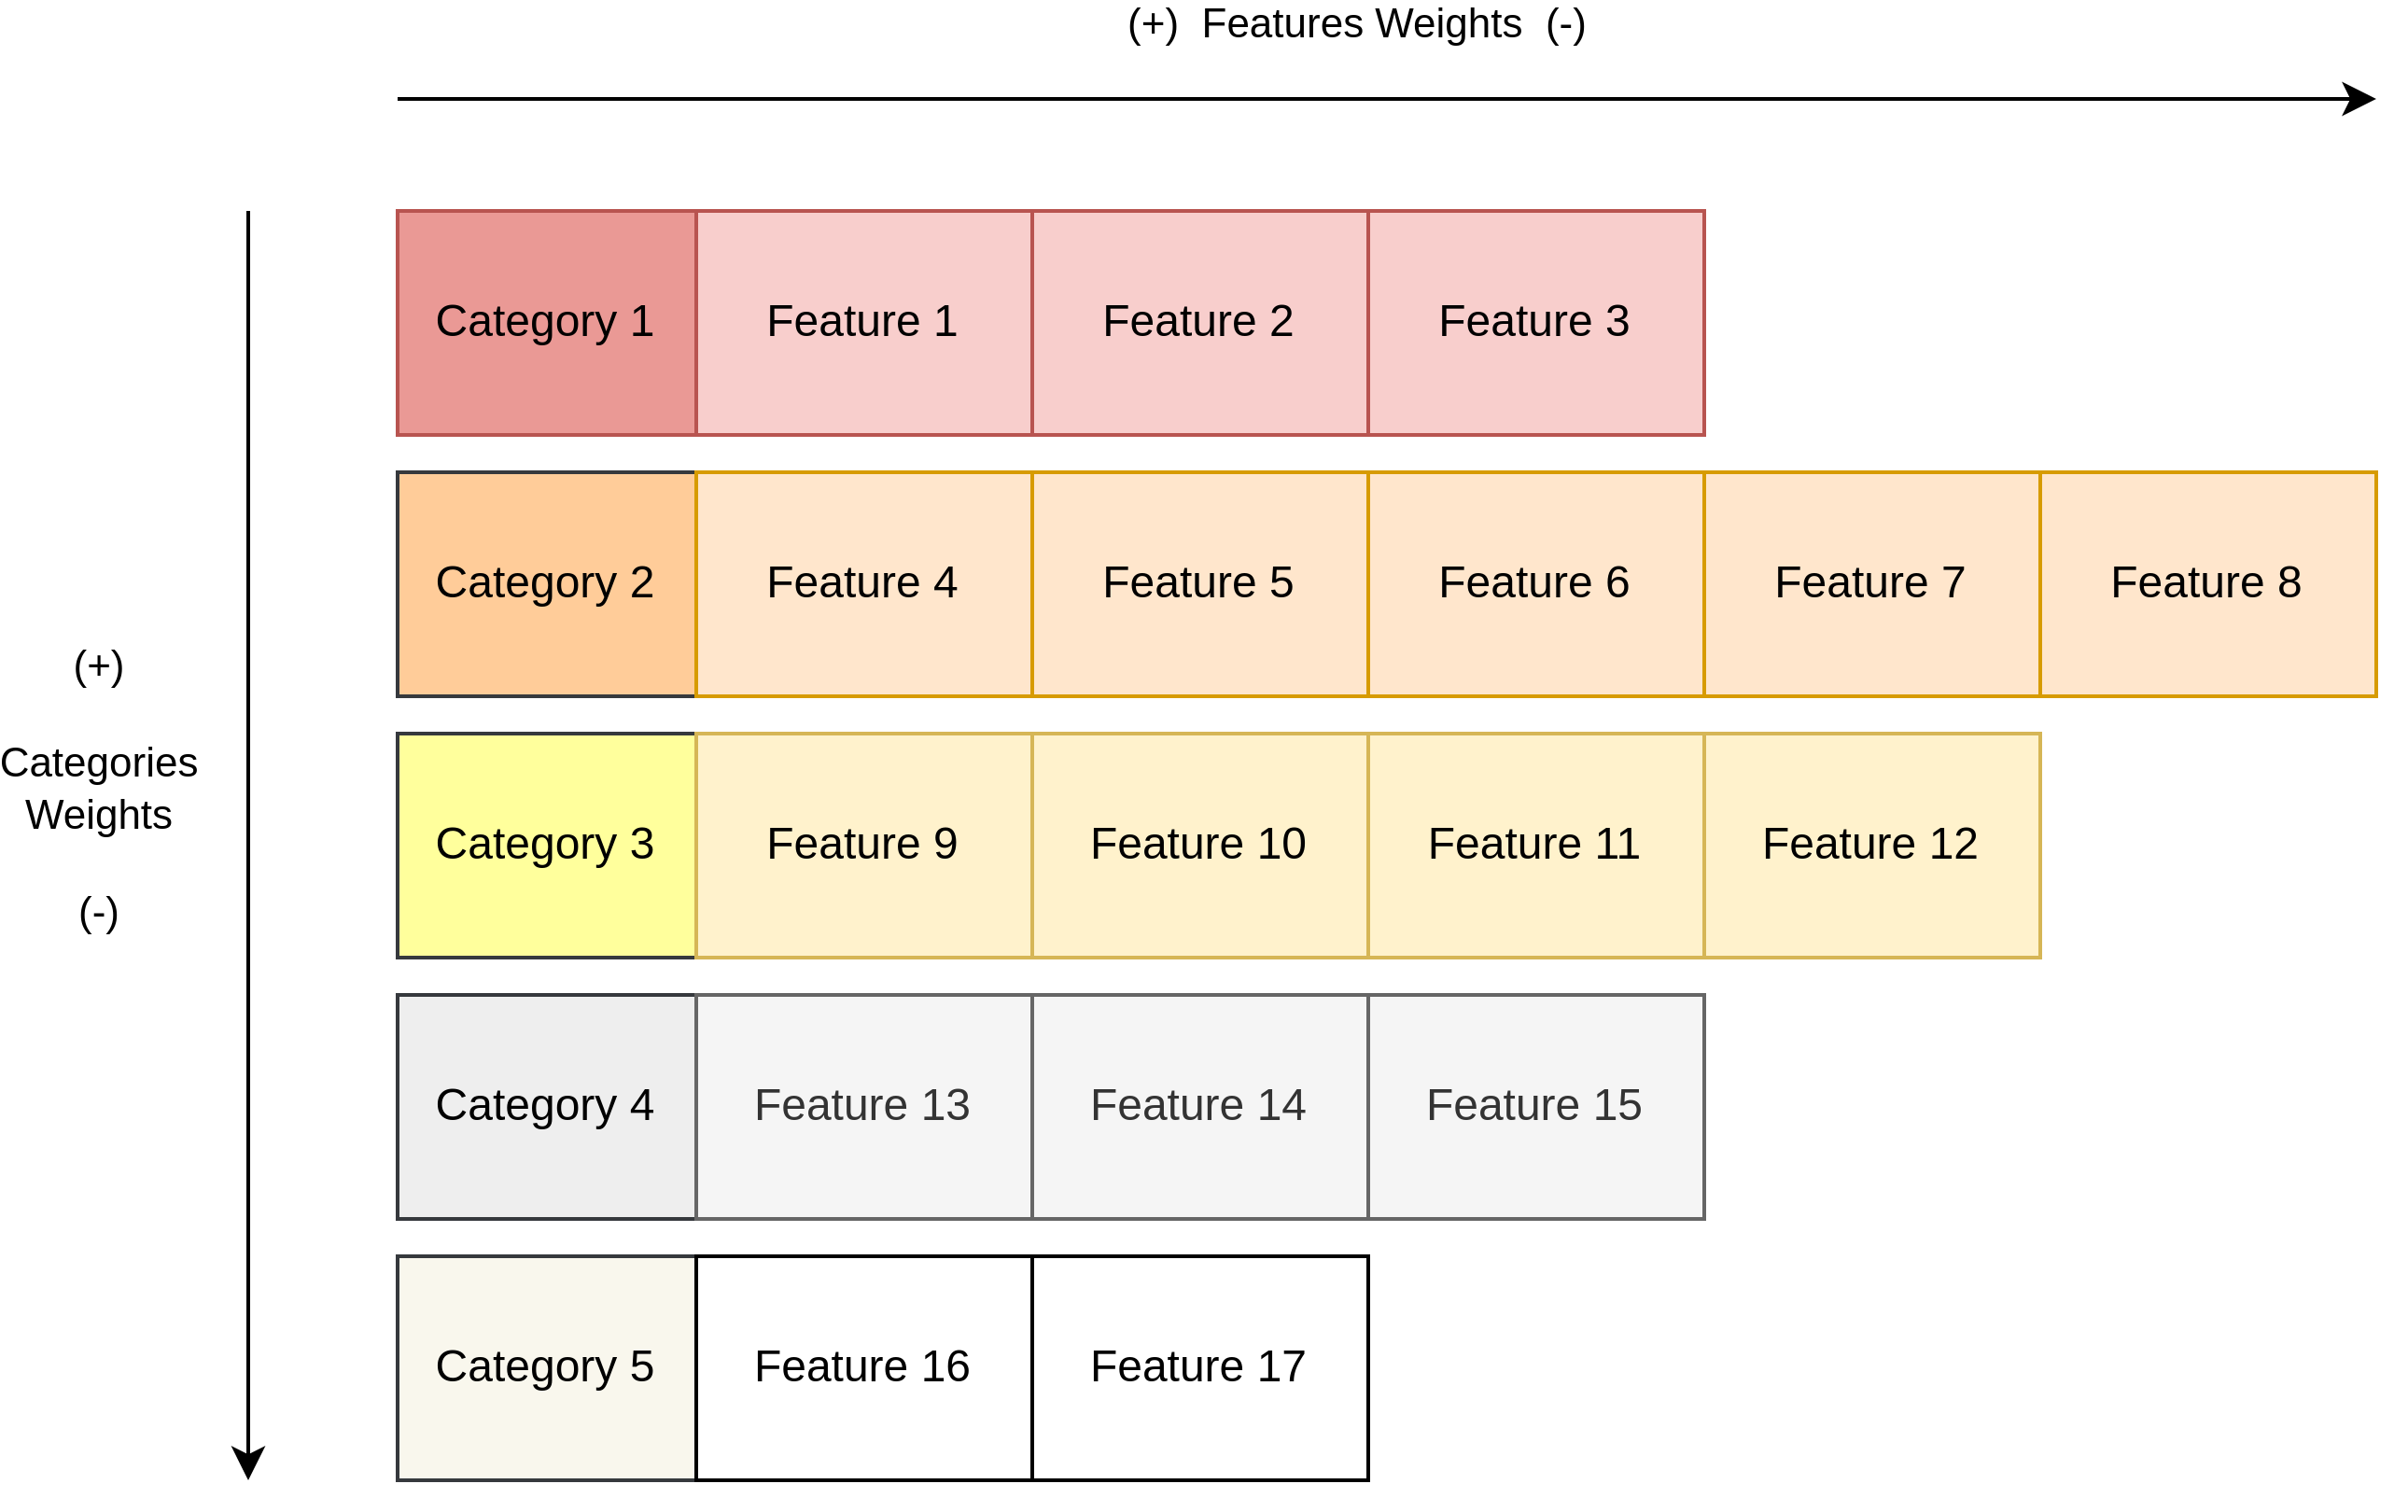
\includegraphics[width=12cm]{Figures/indexing_positions_1_2.png}
	\caption[Asignación de pesos a las categorías en base a las características]{Asignación de pesos a las categorías en base a las características. El peso de las categorías es la suma del peso de las características que la conforman}
	\label{CategoriesFeaturesWeights}
\end{figure}

El resultado de este proceso es una transformación de datos inicialmente tabulares en una matriz $n \times m$, donde $n$ es el número de categorías disponibles en los datos y $m$ es el número de máximo de características que contienen las categorías. Estas matrices están conformadas siguiendo la máxima de que las variables más importantes para los datos se encuentran en las posiciones centrales, como se muestra en la Figura \ref{MatrixIndexes}.


\begin{figure}[H]
	\centering
	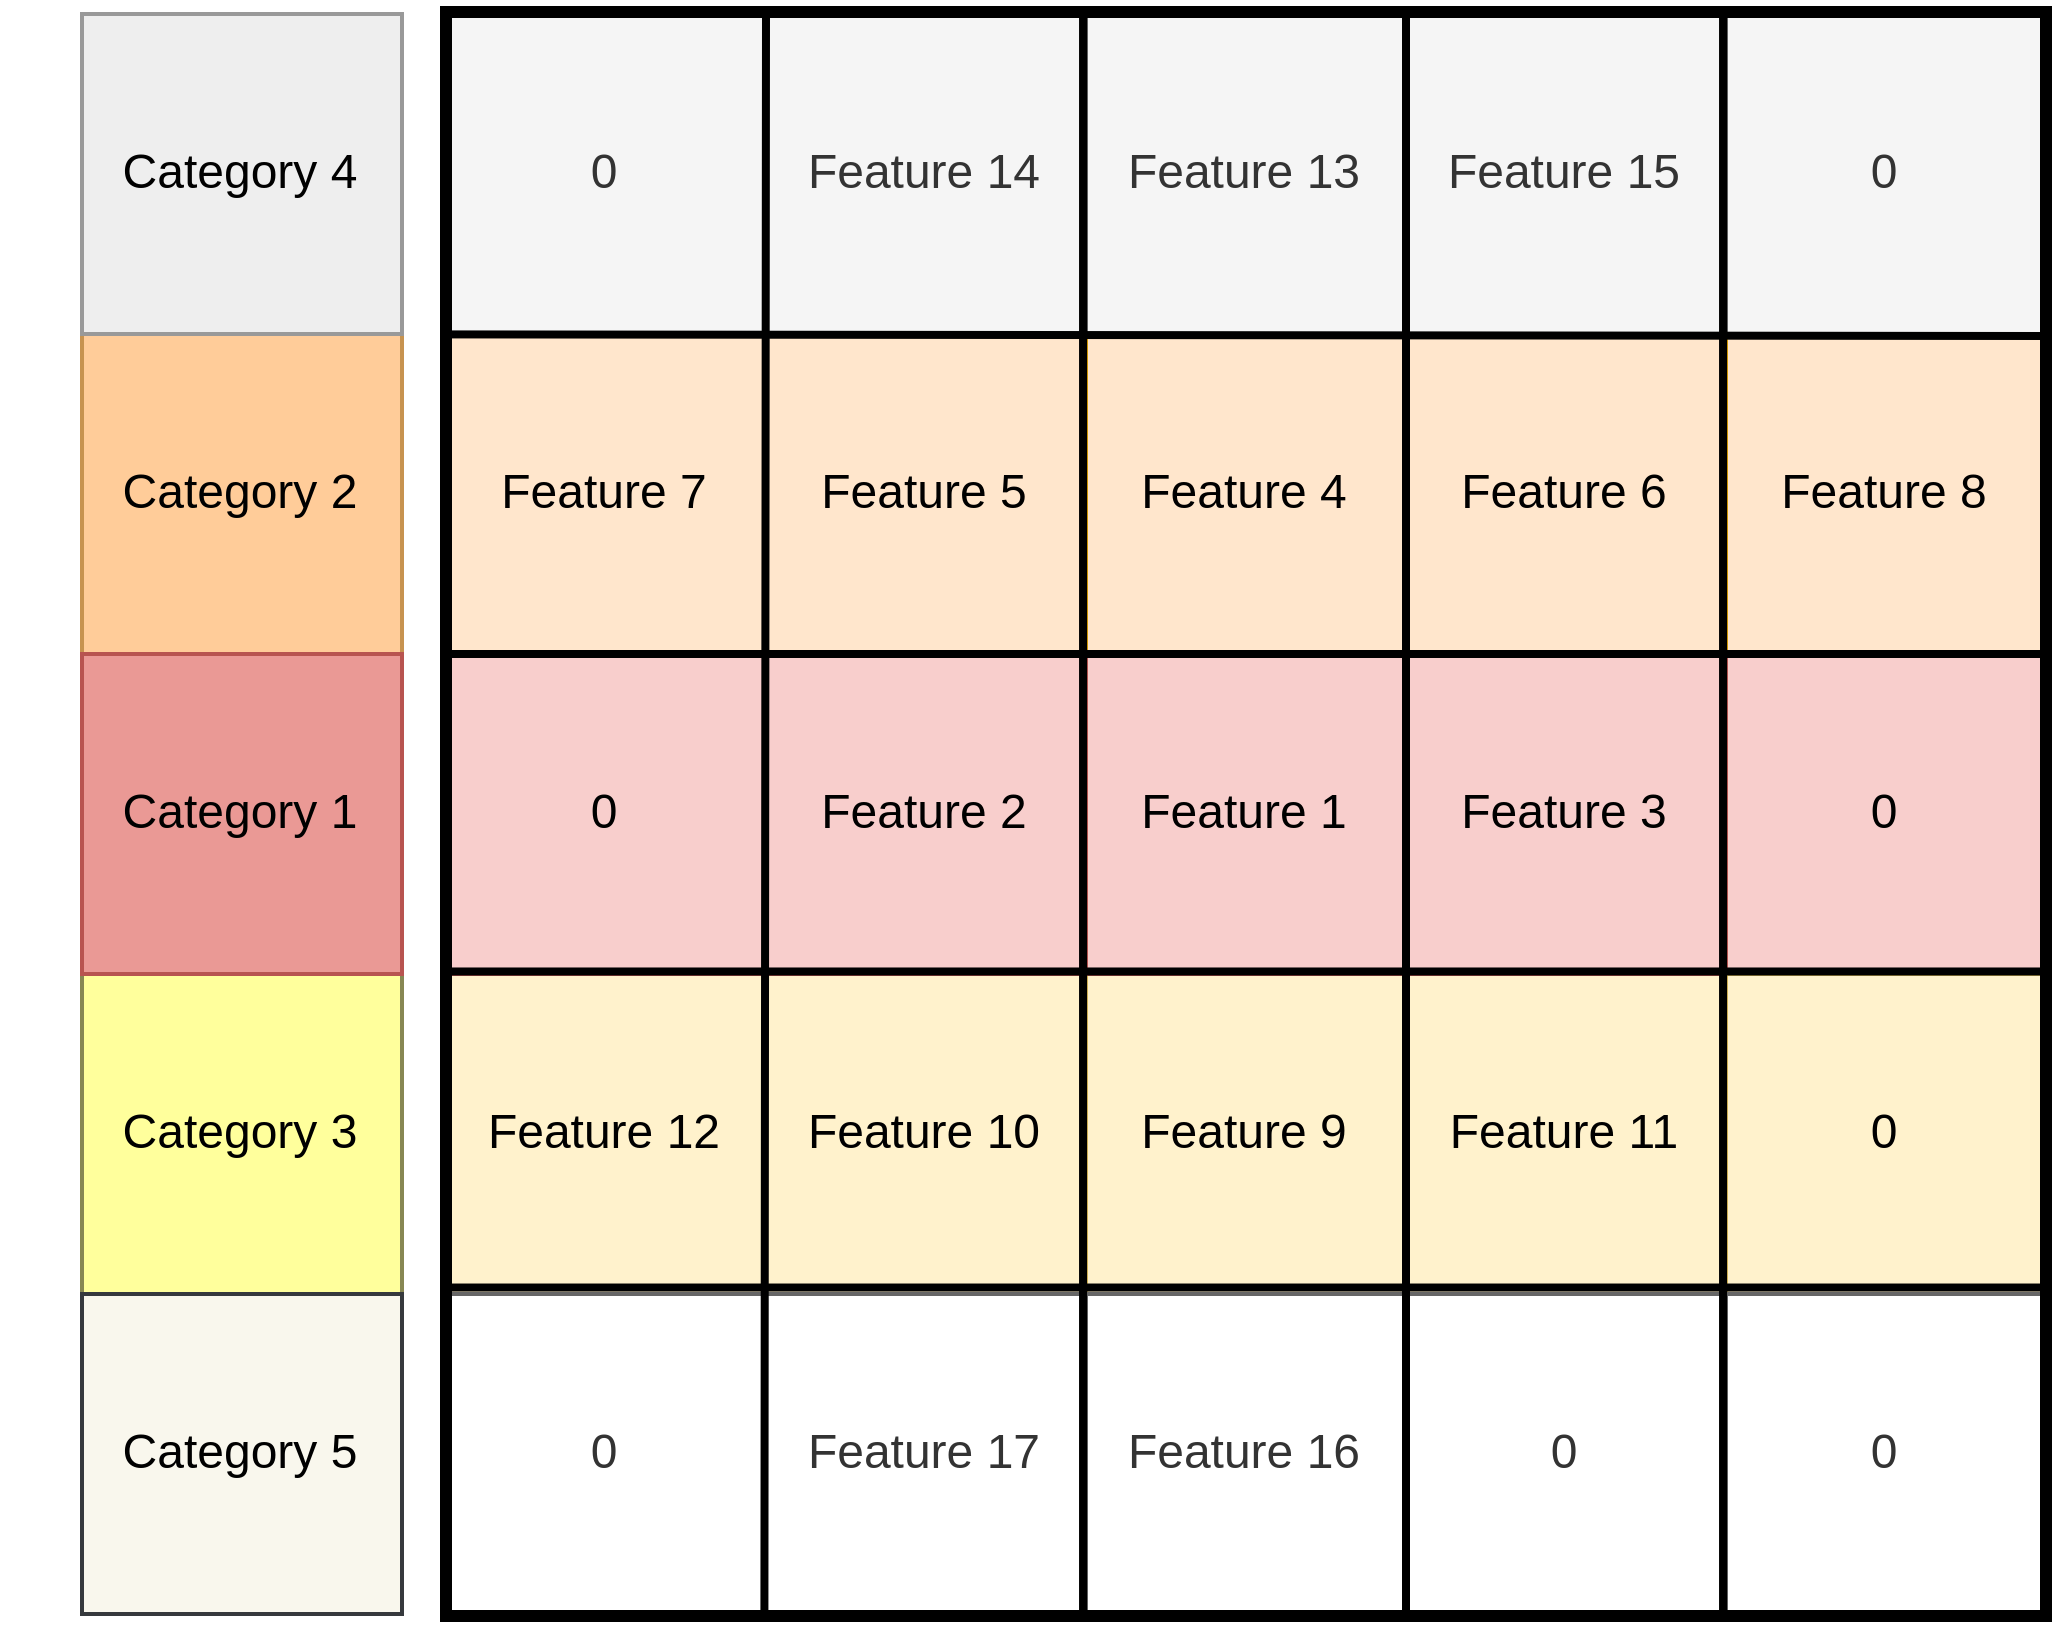
\includegraphics[width=10cm]{Figures/indexing_positions_2.png}
	\caption{Posición de las categorías y características en base a sus pesos}
	\label{MatrixIndexes}
\end{figure}

En la Figura \ref{MatrixConstruction} se muestra un ejemplo de la ejecución de este procedimiento siguiendo el flujo de ejecución del ejemplo de la figura \ref{PostprocessingStage}.

\begin{figure}[H]
	\centering
	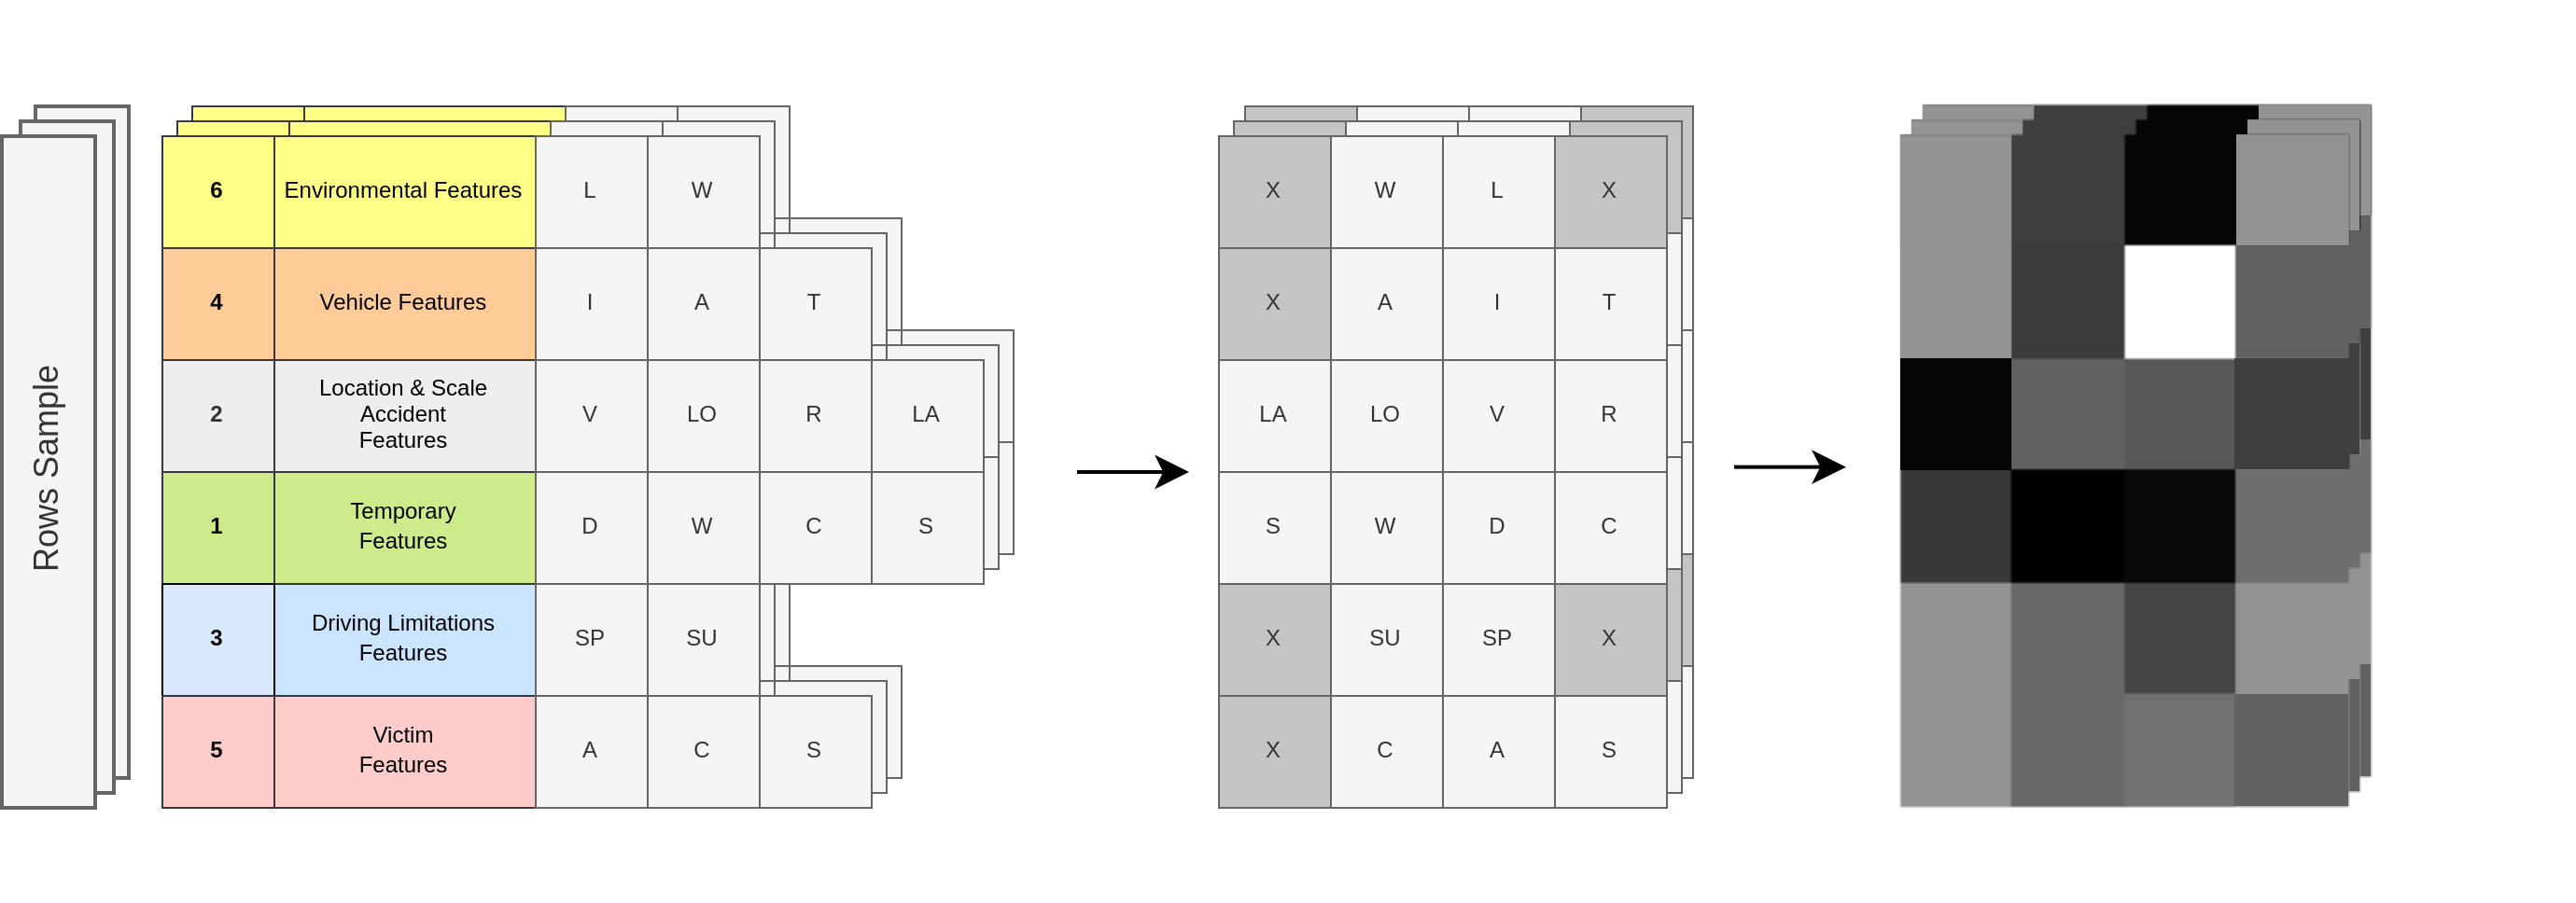
\includegraphics[width=13cm]{Figures/Matrix Construction_2.png}
	\caption[Asignación de características a posiciones de las matrices]{Asignación de características a posiciones de las matrices. Las categorías se asignan a las filas de la matriz en base a su peso; seguidamente, las características de cada categoría se posicionan en las columnas}
	\label{MatrixConstruction}
\end{figure}

\subsubsection{Diseño del modelo}

El nuevo modelo propuesto presenta una arquitectura de cuatro capas convolucionales de dos dimensiones cada una, con un tamaño de \textit{kernel} de $3 \times 3$ y una función de activación \textit{ReLU}. A la salida de cada capa convolucional se aplica un proceso de \textit{Batch Normalization}.

La primera capa convolucional de la red consta de $64$ \textit{kernels}, la segunda de $512$, la tercera de $128$ y la cuarta de $256$. Estos \textit{kernels} contienen los pesos que se entrenan durante la fase de ajuste del modelo a partir de la salida conocida de los datos etiquetados, aprendiendo qué multiplicaciones en los datos minimizan la función de pérdida definida de la red (\textit{Binary Cross Entropy}) gracias al proceso de \textit{Back Propagation}. La salida de cada capa convolucional son los mapas de características (\textit{feature maps}), que son el resultado de aplicar la multiplicación de estos filtros a su entrada. El paso, o número de unidades que avanzan los \textit{kernels}, para un mapa de características, es $1$. También se aplica un relleno en las convoluciones (\textit{padding}), es decir, si la multiplicación del \textit{kernel} excede los límites de la matriz, se agregarán ceros a estos límites para realizar la convolución. Los mapas de características resultantes de la última capa pasan a través de una capa de aplanamiento (\textit{flatten}), que transforma los datos a una sola dimensión una vez que han finalizado las convoluciones. Cada uno de estos datos aplanados está interconectado con los $256$ nodos definidos de la capa densa (\textit{Fully Connected Network}). Finalmente, la capa densa está conectada a una capa final con la función de activación \textit{Softmax}, que da la probabilidad de que cada nueva muestra pertenezca a una de las dos clases. En la figura \ref{CNN2DArchitecture} se puede observar, a modo de diagrama, la arquitectura básica de la red.

\begin{figure}[H]
	\centering
	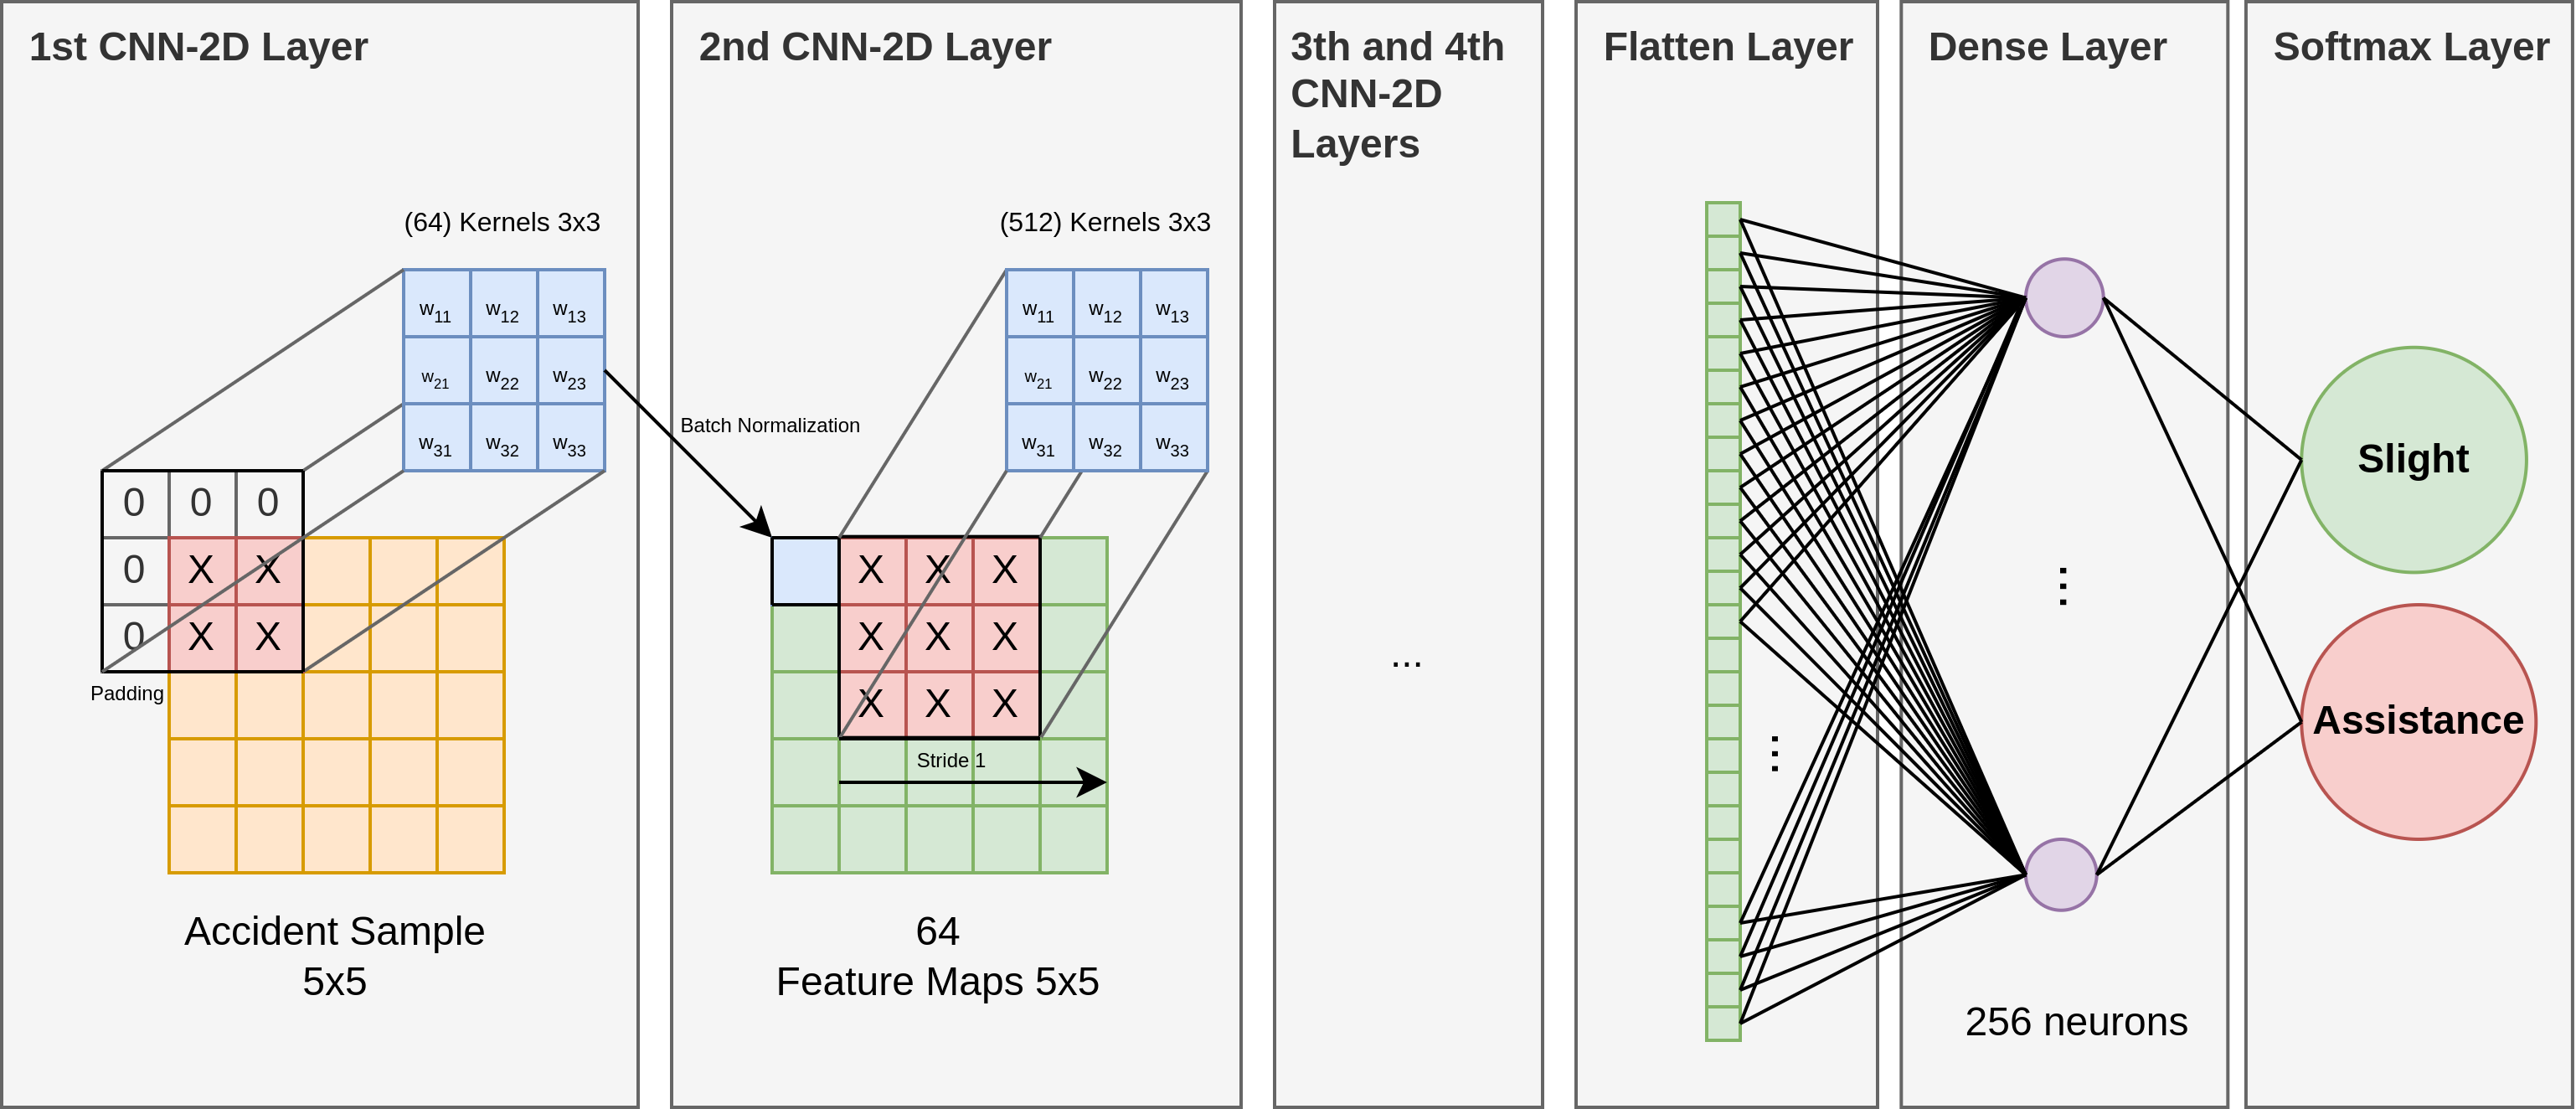
\includegraphics[width=13cm]{Figures/SIMPLE.png}
	\caption{Arquitectura del modelo GTAAF propuesto}
	\label{CNN2DArchitecture}
\end{figure}


\section{Evaluación del modelo: Eficiencia y Robustez}

Para medir el rendimiento y evaluar la capacidad de generalización del modelo GTAAF, se compararán los resultados ofrecidos por este respecto a otros seis modelos de clasificación del estado del arte (\textit{SVC, Naive Bayes, Random Forest, KNN, Regresión Logística y MLP}) a lo largo de tres datasets de accidentes de tráfico de ocho áreas situadas en distintos lugares del mundo. Concretamente España (Madrid), Reino Unido (Southwark, Manchester, Birmingham, Liverpool, Sheffield y Cornwall), y Australia (estado de Victoria).

Con el objetivo de medir la precisión del modelo en distintos contextos, estas regiones han sido seleccionadas debido a que presentan una alta variabilidad, tanto en los datos que contienen, como la extensión de las regiones y en la densidad de población que presentan. De esta forma es posible evaluar el rendimiento del modelo distinguiendo entre tres casos de estudio claramente definidos: (1) alta concentración de población, (2) concentración media y (3) concentración dispersa. Con esta variabilidad en los datos se busca medir la robustez y generalización de la técnica desarrollada.

Por otra parte, se han realizado una serie de experimentos ejecutado el modelo GTAAF sobre los conjuntos de datos eliminando características para comprobar la robustez del modelo. En primer lugar, se prescinde aquella que más relevancia tiene para el modelo (mayor peso), en segundo lugar, aquella que menos relevancia tiene (menor peso) y, en un tercer experimento, quitando ambas. Estas pruebas tienen un doble objetivo: evaluar la robustez del modelo y simular la aplicación del modelo a futuros conjuntos de datos donde no se disponga de valores de todas las características de los conjuntos de datos seleccionados, "eliminando variables significativamente poderosas para los resultados de esta tesis".

Para medir la eficiencia de los modelos se utilizará la métrica \textit{F1-Score}, ya que es una métrica ampliamente utilizada en problemas de clasificación y que representa una buena aproximación a la generalización del modelo, ya que para su cálculo se tienen en cuenta componentes más básicas como la precisión y el recuerdo, indicadores esenciales para una evaluación robusta de cualquier modelo predictivo.
